%%%%%%%%%%%%%%%%%%%%%%%%%%%%%%%%%%%%%%%%%
% Masters/Doctoral Thesis 
% LaTeX Template
% Version 2.5 (27/8/17)
%
% This template was downloaded from:
% http://www.LaTeXTemplates.com
%
% Version 2.x major modifications by:
% Vel (vel@latextemplates.com)
%
% This template is based on a template by:
% Steve Gunn (http://users.ecs.soton.ac.uk/srg/softwaretools/document/templates/)
% Sunil Patel (http://www.sunilpatel.co.uk/thesis-template/)
%
% Template license:
% CC BY-NC-SA 3.0 (http://creativecommons.org/licenses/by-nc-sa/3.0/)
%
%%%%%%%%%%%%%%%%%%%%%%%%%%%%%%%%%%%%%%%%%

%----------------------------------------------------------------------------------------
%	PACKAGES AND OTHER DOCUMENT CONFIGURATIONS
%----------------------------------------------------------------------------------------

\documentclass[
11pt, % The default document font size, options: 10pt, 11pt, 12pt
oneside, % Two side (alternating margins) for binding by default, uncomment to switch to one side
english, % ngerman for German
singlespacing, % Single line spacing, alternatives: onehalfspacing or doublespacing
%draft, % Uncomment to enable draft mode (no pictures, no links, overfull hboxes indicated)
%nolistspacing, % If the document is onehalfspacing or doublespacing, uncomment this to set spacing in lists to single
%liststotoc, % Uncomment to add the list of figures/tables/etc to the table of contents
toctotoc, % Uncomment to add the main table of contents to the table of contents
%parskip, % Uncomment to add space between paragraphs
%nohyperref, % Uncomment to not load the hyperref package
headsepline, % Uncomment to get a line under the header
%chapterinoneline, % Uncomment to place the chapter title next to the number on one line
%consistentlayout, % Uncomment to change the layout of the declaration, abstract and acknowledgements pages to match the default layout
]{MastersDoctoralThesis} % The class file specifying the document structure

\usepackage[utf8]{inputenc} % Required for inputting international characters
\usepackage[T1]{fontenc} % Output font encoding for international characters

\usepackage{mathpazo} % Use the Palatino font by default

\usepackage[backend=bibtex,style=authoryear,natbib=true]{biblatex} % Use the bibtex backend with the authoryear citation style (which resembles APA)

\addbibresource{example.bib} % The filename of the bibliography

\usepackage[autostyle=true]{csquotes} % Required to generate language-dependent quotes in the bibliography

\usepackage{amsmath}
\usepackage{amssymb}
\usepackage{hyperref}
\usepackage{enumitem}
\usepackage{listings}
\usepackage{color}
%\usepackage{natbib}

\usepackage{ntheorem}
\newtheorem*{remark}{Remark}
\newtheorem*{definition}{Definition}

\definecolor{codegreen}{rgb}{0,0.6,0}
\definecolor{codegray}{rgb}{0.5,0.5,0.5}
\definecolor{codepurple}{rgb}{0.58,0,0.82}
\definecolor{backcolour}{gray}{0.85}

\lstdefinestyle{mystyle}{
	backgroundcolor=\color{backcolour},   
	commentstyle=\color{codegreen},
	keywordstyle=\color{magenta},
	numberstyle=\tiny\color{codegray},
	stringstyle=\color{codepurple},
	basicstyle=\footnotesize,
	breakatwhitespace=false,         
	breaklines=true,                 
	captionpos=b,                    
	keepspaces=true,                 
	numbers=left,                    
	numbersep=5pt,                  
	showspaces=false,                
	showstringspaces=false,
	showtabs=false,                  
	tabsize=2
}

\lstset{style=mystyle}

%----------------------------------------------------------------------------------------
%	MARGIN SETTINGS
%----------------------------------------------------------------------------------------

\geometry{
	paper=a4paper, % Change to letterpaper for US letter
	inner=2.5cm, % Inner margin
	outer=3.8cm, % Outer margin
	bindingoffset=.5cm, % Binding offset
	top=1.5cm, % Top margin
	bottom=1.5cm, % Bottom margin
	%showframe, % Uncomment to show how the type block is set on the page
}

%----------------------------------------------------------------------------------------
%	THESIS INFORMATION
%----------------------------------------------------------------------------------------

\thesistitle{Elliptic Curve Hierarchical Deterministic Private Key Sequences: Bitcoin Standards and Best Practices} % Your thesis title, this is used in the title and abstract, print it elsewhere with \ttitle
\supervisor{Prof. Daniele \textsc{Marazzina}\\Prof. Ferdinando M. \textsc{Ametrano} } % Your supervisor's name, this is used in the title page, print it elsewhere with \supname
\examiner{} % Your examiner's name, this is not currently used anywhere in the template, print it elsewhere with \examname
\degree{Mathematical Engeneering} % Your degree name, this is used in the title page and abstract, print it elsewhere with \degreename
\author{Daniele \textsc{Fornaro}} % Your name, this is used in the title page and abstract, print it elsewhere with \authorname
\addresses{} % Your address, this is not currently used anywhere in the template, print it elsewhere with \addressname

\subject{Biological Sciences} % Your subject area, this is not currently used anywhere in the template, print it elsewhere with \subjectname
\keywords{} % Keywords for your thesis, this is not currently used anywhere in the template, print it elsewhere with \keywordnames
\university{\href{https://www.polimi.it}{Politecnico di Milano}} % Your university's name and URL, this is used in the title page and abstract, print it elsewhere with \univname
\department{\href{https://www.mate.polimi.it}{Department of Mathematics}} % Your department's name and URL, this is used in the title page and abstract, print it elsewhere with \deptname
%\group{\href{http://researchgroup.university.com}{Department of Mathematics}} % Your research group's name and URL, this is used in the title page, print it elsewhere with \groupname
\faculty{\href{http://www.ingindinf.polimi.it}{Industrial and Information Engineering}} % Your faculty's name and URL, this is used in the title page and abstract, print it elsewhere with \facname

\AtBeginDocument{
	\hypersetup{pdftitle=\ttitle} % Set the PDF's title to your title
	\hypersetup{pdfauthor=\authorname} % Set the PDF's author to your name
	\hypersetup{pdfkeywords=\keywordnames} % Set the PDF's keywords to your keywords
}

\begin{document}
	
	\frontmatter % Use roman page numbering style (i, ii, iii, iv...) for the pre-content pages
	
	\pagestyle{plain} % Default to the plain heading style until the thesis style is called for the body content
	
	%----------------------------------------------------------------------------------------
	%	TITLE PAGE
	%----------------------------------------------------------------------------------------
	
	\begin{titlepage}
		\begin{center}
			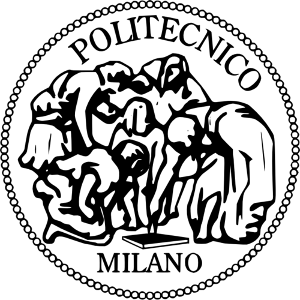
\includegraphics[width=3.5cm]{Logo_Politecnico_Milano} % University/department logo - uncomment to place it
			\\
			\vspace*{.03\textheight}
			{\scshape\LARGE \univname\par}\vspace{1.5cm} % University name
			\textsc{\Large Master Thesis}\\[0.5cm] % Thesis type
			
			\HRule \\[0.4cm] % Horizontal line
			{\huge \bfseries \ttitle\par}\vspace{0.4cm} % Thesis title
			\HRule \\[1.5cm] % Horizontal line
			
			\begin{minipage}[t]{0.35\textwidth}
				\begin{flushleft} \large
					\emph{Author:}\\
					\href{}{\authorname} % Author name - remove the \href bracket to remove the link
				\end{flushleft}
			\end{minipage}
			\begin{minipage}[t]{0.45\textwidth}
				\begin{flushright} \large
					\emph{Supervisors:} \\
					\href{}{\supname} % Supervisor name - remove the \href bracket to remove the link  
				\end{flushright}
			\end{minipage}\\[3cm]
			
			\vfill
			
			\large \textit{A thesis submitted in fulfillment of the requirements\\ for the degree of \degreename}\\[0.3cm] % University requirement text
			\textit{in the}\\[0.4cm]
			\facname\\\deptname\\[2cm] % Research group name and department name
			
			\vfill
			
			{\large 19 April 2018}\\[4cm] % Date
			
			%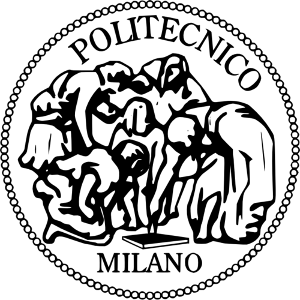
\includegraphics[width=2cm]{Logo_Politecnico_Milano} % University/department logo - uncomment to place it
			
			\vfill
		\end{center}
	\end{titlepage}
	
	%----------------------------------------------------------------------------------------
	%	DECLARATION PAGE
	%----------------------------------------------------------------------------------------
	
%	\begin{declaration}
%	\addchaptertocentry{\authorshipname} % Add the declaration to the table of contents
%	\noindent I, \authorname, declare that this thesis titled, \enquote{\ttitle} and the work presented in it are my own. I confirm that:
	
%	\begin{itemize} 
%		\item This work was done wholly or mainly while in candidature for a research degree at this University.
%		\item Where any part of this thesis has previously been submitted for a degree or any other qualification at this University or any other institution, this has been clearly stated.
%		\item Where I have consulted the published work of others, this is always clearly attributed.
%		\item Where I have quoted from the work of others, the source is always given. With the exception of such quotations, this thesis is entirely my own work.
%		\item I have acknowledged all main sources of help.
%		\item Where the thesis is based on work done by myself jointly with others, I have made clear exactly what was done by others and what I have contributed myself.\\
%	\end{itemize}
	
%	\noindent Signed:\\
%	\rule[0.5em]{25em}{0.5pt} % This prints a line for the signature
	
%	\noindent Date:\\
%	\rule[0.5em]{25em}{0.5pt} % This prints a line to write the date
%\end{declaration}
	
	\cleardoublepage
	
	%----------------------------------------------------------------------------------------
	%	QUOTATION PAGE
	%----------------------------------------------------------------------------------------
	
	\vspace*{0.2\textheight}
	
	\noindent\enquote{\itshape The Times 03/Jan/2009 Chancellor on brink of second bailout for banks}\bigbreak
	
	\hfill Bitcoin Blockchain
	
	%----------------------------------------------------------------------------------------
	%	ABSTRACT PAGE
	%----------------------------------------------------------------------------------------
	
	\begin{abstract}
		\addchaptertocentry{\abstractname} % Add the abstract to the table of contents
		The cryptography used by most of the cryptocurrencies is mainly based on the private-public key pair. The method used to generate private keys is therefore fundamental: it must be efficient, secure and suitable for the situation. Among alternative methods, the Hierarchical Deterministic Wallet has emerged as standard, described in the Bitcoin Improvemnt Proposal #32 (BIP32). Starting from a random number, called SEED, picked up in a sufficiently large range, it is possible to generate numerous private keys in a hierarchical and deterministic way through particular HASH functions and thanks to the elliptic curve properties. Several wallets also use a special algorithm to store the seed and to be able to back it up in a readable form, through the use of a mnemonic phrase, words selected from a specific dictionary. Consensus on a single standard for the mnemonic phrase as not been reached among all major players in the industry yet. This work aims to clarify the various techniques used for the derivation of the keys, with particular attention to the HD wallet. It will also be analyzed the two principal way of encoding the seed, the one described into BIP39 as opposed to the proposal of Electrum, one of the main Bitcoin Wallet, highlighting their respective advantages and disadvantages.
		
	\end{abstract}
	
	%----------------------------------------------------------------------------------------
	%	ACKNOWLEDGEMENTS
	%----------------------------------------------------------------------------------------
	
	\begin{acknowledgements}
		\addchaptertocentry{\acknowledgementname} % Add the acknowledgements to the table of contents
		First of all I would like to give my sincere gratitude to professor Ferdinando Ametrano of the Politecnico di Milano, who transmitted to me the passion of the subject and who has dedicated a large part of his time in order to bring me on the right path. I would like to thank professor Daniele Marazzina of Politecnico di Milano for his supervision to this work and for his many tips. Then I would like to give my thanks to all the friends and colleagues of Deloitte Blockchain Lab Italy for the stimulating and innovative environment in which I was able to write this thesis; in particular Paolo Mazzocchi, Stefano Leone, Raffaele Nicodemo and Calogero Mandracchia, for support and suggestions. Furthermore I would thank Leonardo Comandini for the mutual support and for his help on this work.
		\\ \\
		Finally, I must express my very profound gratitude to my family and to my friends for providing me with unfailing support and continuous encouragement throughout my years of study and through the process of researching and writing this thesis. This accomplishment would not have been possible without them. 
		\\ \\
		Thank you.
	\end{acknowledgements}
	
	%----------------------------------------------------------------------------------------
	%	LIST OF CONTENTS/FIGURES/TABLES PAGES
	%----------------------------------------------------------------------------------------
	\hypersetup{%
		colorlinks = true,
		linkcolor  = black
	}
	\tableofcontents % Prints the main table of contents
	
	%	\listoffigures % Prints the list of figures
	
	%	\listoftables % Prints the list of tables
	
	%----------------------------------------------------------------------------------------
	%	ABBREVIATIONS
	%----------------------------------------------------------------------------------------
	
	%	\begin{abbreviations}{ll} % Include a list of abbreviations (a table of two columns)
	
	%		\textbf{LAH} & \textbf{L}ist \textbf{A}bbreviations \textbf{H}ere\\
	%		\textbf{WSF} & \textbf{W}hat (it) \textbf{S}tands \textbf{F}or\\
	
	%	\end{abbreviations}
	
	%----------------------------------------------------------------------------------------
	%	PHYSICAL CONSTANTS/OTHER DEFINITIONS
	%----------------------------------------------------------------------------------------
	
%	\begin{constants}{lr@{${}={}$}l} % The list of physical constants is a three column table
		
		% The \SI{}{} command is provided by the siunitx package, see its documentation for instructions on how to use it
		
%		Speed of Light & $c_{0}$ & \SI{2.99792458e8}{\meter\per\second} (exact)\\
		%Constant Name & $Symbol$ & $Constant Value$ with units\\
		
%	\end{constants}
	
	%----------------------------------------------------------------------------------------
	%	SYMBOLS
	%----------------------------------------------------------------------------------------
	
%	\begin{symbols}{lll} % Include a list of Symbols (a three column table)
		
%		$a$ & distance & \si{\meter} \\
%		$P$ & power & \si{\watt} (\si{\joule\per\second}) \\
		%Symbol & Name & Unit \\
		
%		\addlinespace % Gap to separate the Roman symbols from the Greek
		
%		$\omega$ & angular frequency & \si{\radian} \\
		
%	\end{symbols}
	
	%----------------------------------------------------------------------------------------
	%	DEDICATION
	%----------------------------------------------------------------------------------------
	
	%\dedicatory{For/Dedicated to/To my\ldots} 
	
	%----------------------------------------------------------------------------------------
	%	THESIS CONTENT - CHAPTERS
	%----------------------------------------------------------------------------------------
	
	\mainmatter % Begin numeric (1,2,3...) page numbering
	
	\pagestyle{thesis} % Return the page headers back to the "thesis" style
	
	% Include the chapters of the thesis as separate files from the Chapters folder
	% Uncomment the lines as you write the chapters
	
	%% Chapter 1

\chapter{Chapter Title Here} % Main chapter title

\label{Chapter1} % For referencing the chapter elsewhere, use \ref{Chapter1} 

%----------------------------------------------------------------------------------------

% Define some commands to keep the formatting separated from the content 
\newcommand{\keyword}[1]{\textbf{#1}}
\newcommand{\tabhead}[1]{\textbf{#1}}
\newcommand{\code}[1]{\texttt{#1}}
\newcommand{\file}[1]{\texttt{\bfseries#1}}
\newcommand{\option}[1]{\texttt{\itshape#1}}

%----------------------------------------------------------------------------------------

\section{Welcome and Thank You}
Welcome to this \LaTeX{} Thesis Template, a beautiful and easy to use template for writing a thesis using the \LaTeX{} typesetting system.

If you are writing a thesis (or will be in the future) and its subject is technical or mathematical (though it doesn't have to be), then creating it in \LaTeX{} is highly recommended as a way to make sure you can just get down to the essential writing without having to worry over formatting or wasting time arguing with your word processor.

\LaTeX{} is easily able to professionally typeset documents that run to hundreds or thousands of pages long. With simple mark-up commands, it automatically sets out the table of contents, margins, page headers and footers and keeps the formatting consistent and beautiful. One of its main strengths is the way it can easily typeset mathematics, even \emph{heavy} mathematics. Even if those equations are the most horribly twisted and most difficult mathematical problems that can only be solved on a super-computer, you can at least count on \LaTeX{} to make them look stunning.

%----------------------------------------------------------------------------------------

\section{Learning \LaTeX{}}

\LaTeX{} is not a \textsc{wysiwyg} (What You See is What You Get) program, unlike word processors such as Microsoft Word or Apple's Pages. Instead, a document written for \LaTeX{} is actually a simple, plain text file that contains \emph{no formatting}. You tell \LaTeX{} how you want the formatting in the finished document by writing in simple commands amongst the text, for example, if I want to use \emph{italic text for emphasis}, I write the \verb|\emph{text}| command and put the text I want in italics in between the curly braces. This means that \LaTeX{} is a \enquote{mark-up} language, very much like HTML.

\subsection{A (not so short) Introduction to \LaTeX{}}

If you are new to \LaTeX{}, there is a very good eBook -- freely available online as a PDF file -- called, \enquote{The Not So Short Introduction to \LaTeX{}}. The book's title is typically shortened to just \emph{lshort}. You can download the latest version (as it is occasionally updated) from here:
\url{http://www.ctan.org/tex-archive/info/lshort/english/lshort.pdf}

It is also available in several other languages. Find yours from the list on this page: \url{http://www.ctan.org/tex-archive/info/lshort/}

It is recommended to take a little time out to learn how to use \LaTeX{} by creating several, small `test' documents, or having a close look at several templates on:\\ 
\url{http://www.LaTeXTemplates.com}\\ 
Making the effort now means you're not stuck learning the system when what you \emph{really} need to be doing is writing your thesis.

\subsection{A Short Math Guide for \LaTeX{}}

If you are writing a technical or mathematical thesis, then you may want to read the document by the AMS (American Mathematical Society) called, \enquote{A Short Math Guide for \LaTeX{}}. It can be found online here:
\url{http://www.ams.org/tex/amslatex.html}
under the \enquote{Additional Documentation} section towards the bottom of the page.

\subsection{Common \LaTeX{} Math Symbols}
There are a multitude of mathematical symbols available for \LaTeX{} and it would take a great effort to learn the commands for them all. The most common ones you are likely to use are shown on this page:
\url{http://www.sunilpatel.co.uk/latex-type/latex-math-symbols/}

You can use this page as a reference or crib sheet, the symbols are rendered as large, high quality images so you can quickly find the \LaTeX{} command for the symbol you need.

\subsection{\LaTeX{} on a Mac}
 
The \LaTeX{} distribution is available for many systems including Windows, Linux and Mac OS X. The package for OS X is called MacTeX and it contains all the applications you need -- bundled together and pre-customized -- for a fully working \LaTeX{} environment and work flow.
 
MacTeX includes a custom dedicated \LaTeX{} editor called TeXShop for writing your `\file{.tex}' files and BibDesk: a program to manage your references and create your bibliography section just as easily as managing songs and creating playlists in iTunes.

%----------------------------------------------------------------------------------------

\section{Getting Started with this Template}

If you are familiar with \LaTeX{}, then you should explore the directory structure of the template and then proceed to place your own information into the \emph{THESIS INFORMATION} block of the \file{main.tex} file. You can then modify the rest of this file to your unique specifications based on your degree/university. Section \ref{FillingFile} on page \pageref{FillingFile} will help you do this. Make sure you also read section \ref{ThesisConventions} about thesis conventions to get the most out of this template.

If you are new to \LaTeX{} it is recommended that you carry on reading through the rest of the information in this document.

Before you begin using this template you should ensure that its style complies with the thesis style guidelines imposed by your institution. In most cases this template style and layout will be suitable. If it is not, it may only require a small change to bring the template in line with your institution's recommendations. These modifications will need to be done on the \file{MastersDoctoralThesis.cls} file.

\subsection{About this Template}

This \LaTeX{} Thesis Template is originally based and created around a \LaTeX{} style file created by Steve R.\ Gunn from the University of Southampton (UK), department of Electronics and Computer Science. You can find his original thesis style file at his site, here:
\url{http://www.ecs.soton.ac.uk/~srg/softwaretools/document/templates/}

Steve's \file{ecsthesis.cls} was then taken by Sunil Patel who modified it by creating a skeleton framework and folder structure to place the thesis files in. The resulting template can be found on Sunil's site here:
\url{http://www.sunilpatel.co.uk/thesis-template}

Sunil's template was made available through \url{http://www.LaTeXTemplates.com} where it was modified many times based on user requests and questions. Version 2.0 and onwards of this template represents a major modification to Sunil's template and is, in fact, hardly recognisable. The work to make version 2.0 possible was carried out by \href{mailto:vel@latextemplates.com}{Vel} and Johannes Böttcher.

%----------------------------------------------------------------------------------------

\section{What this Template Includes}

\subsection{Folders}

This template comes as a single zip file that expands out to several files and folders. The folder names are mostly self-explanatory:

\keyword{Appendices} -- this is the folder where you put the appendices. Each appendix should go into its own separate \file{.tex} file. An example and template are included in the directory.

\keyword{Chapters} -- this is the folder where you put the thesis chapters. A thesis usually has about six chapters, though there is no hard rule on this. Each chapter should go in its own separate \file{.tex} file and they can be split as:
\begin{itemize}
\item Chapter 1: Introduction to the thesis topic
\item Chapter 2: Background information and theory
\item Chapter 3: (Laboratory) experimental setup
\item Chapter 4: Details of experiment 1
\item Chapter 5: Details of experiment 2
\item Chapter 6: Discussion of the experimental results
\item Chapter 7: Conclusion and future directions
\end{itemize}
This chapter layout is specialised for the experimental sciences, your discipline may be different.

\keyword{Figures} -- this folder contains all figures for the thesis. These are the final images that will go into the thesis document.

\subsection{Files}

Included are also several files, most of them are plain text and you can see their contents in a text editor. After initial compilation, you will see that more auxiliary files are created by \LaTeX{} or BibTeX and which you don't need to delete or worry about:

\keyword{example.bib} -- this is an important file that contains all the bibliographic information and references that you will be citing in the thesis for use with BibTeX. You can write it manually, but there are reference manager programs available that will create and manage it for you. Bibliographies in \LaTeX{} are a large subject and you may need to read about BibTeX before starting with this. Many modern reference managers will allow you to export your references in BibTeX format which greatly eases the amount of work you have to do.

\keyword{MastersDoctoralThesis.cls} -- this is an important file. It is the class file that tells \LaTeX{} how to format the thesis. 

\keyword{main.pdf} -- this is your beautifully typeset thesis (in the PDF file format) created by \LaTeX{}. It is supplied in the PDF with the template and after you compile the template you should get an identical version.

\keyword{main.tex} -- this is an important file. This is the file that you tell \LaTeX{} to compile to produce your thesis as a PDF file. It contains the framework and constructs that tell \LaTeX{} how to layout the thesis. It is heavily commented so you can read exactly what each line of code does and why it is there. After you put your own information into the \emph{THESIS INFORMATION} block -- you have now started your thesis!

Files that are \emph{not} included, but are created by \LaTeX{} as auxiliary files include:

\keyword{main.aux} -- this is an auxiliary file generated by \LaTeX{}, if it is deleted \LaTeX{} simply regenerates it when you run the main \file{.tex} file.

\keyword{main.bbl} -- this is an auxiliary file generated by BibTeX, if it is deleted, BibTeX simply regenerates it when you run the \file{main.aux} file. Whereas the \file{.bib} file contains all the references you have, this \file{.bbl} file contains the references you have actually cited in the thesis and is used to build the bibliography section of the thesis.

\keyword{main.blg} -- this is an auxiliary file generated by BibTeX, if it is deleted BibTeX simply regenerates it when you run the main \file{.aux} file.

\keyword{main.lof} -- this is an auxiliary file generated by \LaTeX{}, if it is deleted \LaTeX{} simply regenerates it when you run the main \file{.tex} file. It tells \LaTeX{} how to build the \emph{List of Figures} section.

\keyword{main.log} -- this is an auxiliary file generated by \LaTeX{}, if it is deleted \LaTeX{} simply regenerates it when you run the main \file{.tex} file. It contains messages from \LaTeX{}, if you receive errors and warnings from \LaTeX{}, they will be in this \file{.log} file.

\keyword{main.lot} -- this is an auxiliary file generated by \LaTeX{}, if it is deleted \LaTeX{} simply regenerates it when you run the main \file{.tex} file. It tells \LaTeX{} how to build the \emph{List of Tables} section.

\keyword{main.out} -- this is an auxiliary file generated by \LaTeX{}, if it is deleted \LaTeX{} simply regenerates it when you run the main \file{.tex} file.

So from this long list, only the files with the \file{.bib}, \file{.cls} and \file{.tex} extensions are the most important ones. The other auxiliary files can be ignored or deleted as \LaTeX{} and BibTeX will regenerate them.

%----------------------------------------------------------------------------------------

\section{Filling in Your Information in the \file{main.tex} File}\label{FillingFile}

You will need to personalise the thesis template and make it your own by filling in your own information. This is done by editing the \file{main.tex} file in a text editor or your favourite LaTeX environment.

Open the file and scroll down to the third large block titled \emph{THESIS INFORMATION} where you can see the entries for \emph{University Name}, \emph{Department Name}, etc \ldots

Fill out the information about yourself, your group and institution. You can also insert web links, if you do, make sure you use the full URL, including the \code{http://} for this. If you don't want these to be linked, simply remove the \verb|\href{url}{name}| and only leave the name.

When you have done this, save the file and recompile \code{main.tex}. All the information you filled in should now be in the PDF, complete with web links. You can now begin your thesis proper!

%----------------------------------------------------------------------------------------

\section{The \code{main.tex} File Explained}

The \file{main.tex} file contains the structure of the thesis. There are plenty of written comments that explain what pages, sections and formatting the \LaTeX{} code is creating. Each major document element is divided into commented blocks with titles in all capitals to make it obvious what the following bit of code is doing. Initially there seems to be a lot of \LaTeX{} code, but this is all formatting, and it has all been taken care of so you don't have to do it.

Begin by checking that your information on the title page is correct. For the thesis declaration, your institution may insist on something different than the text given. If this is the case, just replace what you see with what is required in the \emph{DECLARATION PAGE} block.

Then comes a page which contains a funny quote. You can put your own, or quote your favourite scientist, author, person, and so on. Make sure to put the name of the person who you took the quote from.

Following this is the abstract page which summarises your work in a condensed way and can almost be used as a standalone document to describe what you have done. The text you write will cause the heading to move up so don't worry about running out of space.

Next come the acknowledgements. On this page, write about all the people who you wish to thank (not forgetting parents, partners and your advisor/supervisor).

The contents pages, list of figures and tables are all taken care of for you and do not need to be manually created or edited. The next set of pages are more likely to be optional and can be deleted since they are for a more technical thesis: insert a list of abbreviations you have used in the thesis, then a list of the physical constants and numbers you refer to and finally, a list of mathematical symbols used in any formulae. Making the effort to fill these tables means the reader has a one-stop place to refer to instead of searching the internet and references to try and find out what you meant by certain abbreviations or symbols.

The list of symbols is split into the Roman and Greek alphabets. Whereas the abbreviations and symbols ought to be listed in alphabetical order (and this is \emph{not} done automatically for you) the list of physical constants should be grouped into similar themes.

The next page contains a one line dedication. Who will you dedicate your thesis to?

Finally, there is the block where the chapters are included. Uncomment the lines (delete the \code{\%} character) as you write the chapters. Each chapter should be written in its own file and put into the \emph{Chapters} folder and named \file{Chapter1}, \file{Chapter2}, etc\ldots Similarly for the appendices, uncomment the lines as you need them. Each appendix should go into its own file and placed in the \emph{Appendices} folder.

After the preamble, chapters and appendices finally comes the bibliography. The bibliography style (called \option{authoryear}) is used for the bibliography and is a fully featured style that will even include links to where the referenced paper can be found online. Do not underestimate how grateful your reader will be to find that a reference to a paper is just a click away. Of course, this relies on you putting the URL information into the BibTeX file in the first place.

%----------------------------------------------------------------------------------------

\section{Thesis Features and Conventions}\label{ThesisConventions}

To get the best out of this template, there are a few conventions that you may want to follow.

One of the most important (and most difficult) things to keep track of in such a long document as a thesis is consistency. Using certain conventions and ways of doing things (such as using a Todo list) makes the job easier. Of course, all of these are optional and you can adopt your own method.

\subsection{Printing Format}

This thesis template is designed for double sided printing (i.e. content on the front and back of pages) as most theses are printed and bound this way. Switching to one sided printing is as simple as uncommenting the \option{oneside} option of the \code{documentclass} command at the top of the \file{main.tex} file. You may then wish to adjust the margins to suit specifications from your institution.

The headers for the pages contain the page number on the outer side (so it is easy to flick through to the page you want) and the chapter name on the inner side.

The text is set to 11 point by default with single line spacing, again, you can tune the text size and spacing should you want or need to using the options at the very start of \file{main.tex}. The spacing can be changed similarly by replacing the \option{singlespacing} with \option{onehalfspacing} or \option{doublespacing}.

\subsection{Using US Letter Paper}

The paper size used in the template is A4, which is the standard size in Europe. If you are using this thesis template elsewhere and particularly in the United States, then you may have to change the A4 paper size to the US Letter size. This can be done in the margins settings section in \file{main.tex}.

Due to the differences in the paper size, the resulting margins may be different to what you like or require (as it is common for institutions to dictate certain margin sizes). If this is the case, then the margin sizes can be tweaked by modifying the values in the same block as where you set the paper size. Now your document should be set up for US Letter paper size with suitable margins.

\subsection{References}

The \code{biblatex} package is used to format the bibliography and inserts references such as this one \parencite{Reference1}. The options used in the \file{main.tex} file mean that the in-text citations of references are formatted with the author(s) listed with the date of the publication. Multiple references are separated by semicolons (e.g. \parencite{Reference2, Reference1}) and references with more than three authors only show the first author with \emph{et al.} indicating there are more authors (e.g. \parencite{Reference3}). This is done automatically for you. To see how you use references, have a look at the \file{Chapter1.tex} source file. Many reference managers allow you to simply drag the reference into the document as you type.

Scientific references should come \emph{before} the punctuation mark if there is one (such as a comma or period). The same goes for footnotes\footnote{Such as this footnote, here down at the bottom of the page.}. You can change this but the most important thing is to keep the convention consistent throughout the thesis. Footnotes themselves should be full, descriptive sentences (beginning with a capital letter and ending with a full stop). The APA6 states: \enquote{Footnote numbers should be superscripted, [...], following any punctuation mark except a dash.} The Chicago manual of style states: \enquote{A note number should be placed at the end of a sentence or clause. The number follows any punctuation mark except the dash, which it precedes. It follows a closing parenthesis.}

The bibliography is typeset with references listed in alphabetical order by the first author's last name. This is similar to the APA referencing style. To see how \LaTeX{} typesets the bibliography, have a look at the very end of this document (or just click on the reference number links in in-text citations).

\subsubsection{A Note on bibtex}

The bibtex backend used in the template by default does not correctly handle unicode character encoding (i.e. "international" characters). You may see a warning about this in the compilation log and, if your references contain unicode characters, they may not show up correctly or at all. The solution to this is to use the biber backend instead of the outdated bibtex backend. This is done by finding this in \file{main.tex}: \option{backend=bibtex} and changing it to \option{backend=biber}. You will then need to delete all auxiliary BibTeX files and navigate to the template directory in your terminal (command prompt). Once there, simply type \code{biber main} and biber will compile your bibliography. You can then compile \file{main.tex} as normal and your bibliography will be updated. An alternative is to set up your LaTeX editor to compile with biber instead of bibtex, see \href{http://tex.stackexchange.com/questions/154751/biblatex-with-biber-configuring-my-editor-to-avoid-undefined-citations/}{here} for how to do this for various editors.

\subsection{Tables}

Tables are an important way of displaying your results, below is an example table which was generated with this code:

{\small
\begin{verbatim}
\begin{table}
\caption{The effects of treatments X and Y on the four groups studied.}
\label{tab:treatments}
\centering
\begin{tabular}{l l l}
\toprule
\tabhead{Groups} & \tabhead{Treatment X} & \tabhead{Treatment Y} \\
\midrule
1 & 0.2 & 0.8\\
2 & 0.17 & 0.7\\
3 & 0.24 & 0.75\\
4 & 0.68 & 0.3\\
\bottomrule\\
\end{tabular}
\end{table}
\end{verbatim}
}

\begin{table}
\caption{The effects of treatments X and Y on the four groups studied.}
\label{tab:treatments}
\centering
\begin{tabular}{l l l}
\toprule
\tabhead{Groups} & \tabhead{Treatment X} & \tabhead{Treatment Y} \\
\midrule
1 & 0.2 & 0.8\\
2 & 0.17 & 0.7\\
3 & 0.24 & 0.75\\
4 & 0.68 & 0.3\\
\bottomrule\\
\end{tabular}
\end{table}

You can reference tables with \verb|\ref{<label>}| where the label is defined within the table environment. See \file{Chapter1.tex} for an example of the label and citation (e.g. Table~\ref{tab:treatments}).

\subsection{Figures}

There will hopefully be many figures in your thesis (that should be placed in the \emph{Figures} folder). The way to insert figures into your thesis is to use a code template like this:
\begin{verbatim}
\begin{figure}
\centering

\includegraphics{Figures/Electron}
\decoRule
\caption[An Electron]{An electron (artist's impression).}
\label{fig:Electron}
\end{figure}
\end{verbatim}
Also look in the source file. Putting this code into the source file produces the picture of the electron that you can see in the figure below.

\begin{figure}[th]
\centering

\includegraphics{Figures/Electron}
\decoRule
\caption[An Electron]{An electron (artist's impression).}
\label{fig:Electron}
\end{figure}

Sometimes figures don't always appear where you write them in the source. The placement depends on how much space there is on the page for the figure. Sometimes there is not enough room to fit a figure directly where it should go (in relation to the text) and so \LaTeX{} puts it at the top of the next page. Positioning figures is the job of \LaTeX{} and so you should only worry about making them look good!

Figures usually should have captions just in case you need to refer to them (such as in Figure~\ref{fig:Electron}). The \verb|\caption| command contains two parts, the first part, inside the square brackets is the title that will appear in the \emph{List of Figures}, and so should be short. The second part in the curly brackets should contain the longer and more descriptive caption text.

The \verb|\decoRule| command is optional and simply puts an aesthetic horizontal line below the image. If you do this for one image, do it for all of them.

\LaTeX{} is capable of using images in pdf, jpg and png format.

\subsection{Typesetting mathematics}

If your thesis is going to contain heavy mathematical content, be sure that \LaTeX{} will make it look beautiful, even though it won't be able to solve the equations for you.

The \enquote{Not So Short Introduction to \LaTeX} (available on \href{http://www.ctan.org/tex-archive/info/lshort/english/lshort.pdf}{CTAN}) should tell you everything you need to know for most cases of typesetting mathematics. If you need more information, a much more thorough mathematical guide is available from the AMS called, \enquote{A Short Math Guide to \LaTeX} and can be downloaded from:
\url{ftp://ftp.ams.org/pub/tex/doc/amsmath/short-math-guide.pdf}

There are many different \LaTeX{} symbols to remember, luckily you can find the most common symbols in \href{http://ctan.org/pkg/comprehensive}{The Comprehensive \LaTeX~Symbol List}.

You can write an equation, which is automatically given an equation number by \LaTeX{} like this:
\begin{verbatim}
\begin{equation}
E = mc^{2}
\label{eqn:Einstein}
\end{equation}
\end{verbatim}

This will produce Einstein's famous energy-matter equivalence equation:
\begin{equation}
E = mc^{2}
\label{eqn:Einstein}
\end{equation}

All equations you write (which are not in the middle of paragraph text) are automatically given equation numbers by \LaTeX{}. If you don't want a particular equation numbered, use the unnumbered form:
\begin{verbatim}
\[ a^{2}=4 \]
\end{verbatim}

%----------------------------------------------------------------------------------------

\section{Sectioning and Subsectioning}

You should break your thesis up into nice, bite-sized sections and subsections. \LaTeX{} automatically builds a table of Contents by looking at all the \verb|\chapter{}|, \verb|\section{}|  and \verb|\subsection{}| commands you write in the source.

The Table of Contents should only list the sections to three (3) levels. A \verb|chapter{}| is level zero (0). A \verb|\section{}| is level one (1) and so a \verb|\subsection{}| is level two (2). In your thesis it is likely that you will even use a \verb|subsubsection{}|, which is level three (3). The depth to which the Table of Contents is formatted is set within \file{MastersDoctoralThesis.cls}. If you need this changed, you can do it in \file{main.tex}.

%----------------------------------------------------------------------------------------

\section{In Closing}

You have reached the end of this mini-guide. You can now rename or overwrite this pdf file and begin writing your own \file{Chapter1.tex} and the rest of your thesis. The easy work of setting up the structure and framework has been taken care of for you. It's now your job to fill it out!

Good luck and have lots of fun!

\begin{flushright}
Guide written by ---\\
Sunil Patel: \href{http://www.sunilpatel.co.uk}{www.sunilpatel.co.uk}\\
Vel: \href{http://www.LaTeXTemplates.com}{LaTeXTemplates.com}
\end{flushright}

	% Chapter 1

\chapter*{Introduction} % Main chapter title
\addcontentsline{toc}{chapter}{Introduction}
\label{Introduction} % For referencing the chapter elsewhere, use \ref{Chapter1} 

%----------------------------------------------------------------------------------------

% Define some commands to keep the formatting separated from the content 
%----------------------------------------------------------------------------------------
The cryptography used by most of the cryptocurrencies is mainly based on the private-public key pair. It is therefore fundamental the method used to generate private keys, which must be efficient, secure and suitable for the situation.
\\ \\
This thesis claims to analyze in detail the principal techniques used for the derivation of the public-private keys pair in the Bitcoin framework.
\\ \\
The first chapter will give an explanation of the basic concepts needed for this work. Two fundamental elements are used: HASH functions and the Elliptic Curve. The former are irreversible algorithms; although the image of such functions is a limited set, it doesn't exist an analytic expression for the inverse. The only way to compute the inverse of a hash function is by trying and this will take to much time, due to high computational costs, making the operation infeasible.
The latter, the Elliptic Curve, is defined by an equation over a specific field and it is a plane algebraic curve in this contest. In this type of cryptography a point on this curve is called public key and the integer number, used to obtain the point, is called private key. In this chapter, all the most important properties of this curve will be explained.
\\ \\
In the second chapter will be analyzed in detail the principal techniques used in order to generate private and public key pairs. In particular, we will see four type of derivations. The first and naive method consists of randomly extracting a number and considering it as a private key, from which the corresponding public key will be generated each time a new pair is requested. The other three methods are the so-called: \textit{deterministic}. This is due to the fact that in order to generate a bunch of keys, it is necessary one single datum, called \textit{seed}. These three methods are in an increasing scale of difficulty and complexity and we will see their principal advantages and disadvantages. The last type of derivation is the most used because it derives the keys in a hierarchical way. This method will be seen in the next chapter.
\\ \\
The third chapter will be focused on the analysis of the Hierarchical Deterministic Wallet, the most sophisticated type of derivation used up to now. It is defined by BIP32 [\cite{1}] and it is used by most of the Bitcoin wallets. This derivation is deterministic, a seed is needed, and it is hierarchical. From the seed it is possible to derive a large number of keys and all of these keys can derive new keys in the same way and so on. This procedure can be iterated as long as desired, leaving the user a wide choice in the derivation of these numbers.
\\ \\
In the fourth chapter there will be the analysis of two possible ways to store the seed: one was proposed by BIP39 [\cite{2}] and it is the most used in the Bitcoin framework; the other is the one used by Electrum [\cite{3}], one of the principal Bitcoin wallet. Both of them used a mnemonic phrase, a sentence composed of a certain number of words from which it is possible to derive the seed. Nevertheless, they have some differences and we will analyze them. The principal difference stands in the different way used to verify the correctness of the mnemonic phrase. With BIP32 it is only possible to check if the phrase is plausible, but with Electrum it is possible to assign a version to the seed that will be generated by the mnemonic phrase, giving a purpose to the keys derived from it.
\\ \\
The fifth chapter will be focused on some possible applications of the Hierarchical Deterministic Wallet proposed by BIP32. In particular we will see the standard way to write a \textit{path}, in order to easily understand how to generate particular keys from the seed.  We will also analyze one of the standards used by most of the Bitcoin wallet: BIP43 [\cite{4}]. The purpose of this BIP is to give a particular meaning to some branches of the tree. We will therefore describe two important applications: multi-coin wallet BIP44 [\cite{5}] and SegWit addresses BIP49 [\cite{6}].
\\ \\
In the appendix there will be a summary of methods used for the representation of private and public keys in the Bitcoin framework and respective addresses.
\\ \\
Along with this writing, I attach the GitHub link to the repository of python code for the course of professor F. Ametrano. In this repository I have replicated in python all the procedures and methods presented and described in this thesis, neglecting all those parts that are not inherent to it and writing the important ones in a synthetic and essential way.
\\ \\
\hypersetup{
	colorlinks=true,
	urlcolor=black
}
\href{https://github.com/fametrano/BitcoinBlockchainTechnology}{\texttt{https://github.com/fametrano/BitcoinBlockchainTechnology}}

	% Chapter 1

\chapter{Cryptography} % Main chapter title

\label{EC} % For referencing the chapter elsewhere, use \ref{Chapter1} 

%----------------------------------------------------------------------------------------

% Define some commands to keep the formatting separated from the content 
\newcommand{\keyword}[1]{\textbf{#1}}
\newcommand{\tabhead}[1]{\textbf{#1}}
\newcommand{\code}[1]{\texttt{#1}}
\newcommand{\file}[1]{\texttt{\bfseries#1}}
\newcommand{\option}[1]{\texttt{\itshape#1}}

%----------------------------------------------------------------------------------------

In order to have a clear understanding of this thesis, it is necessary to know the basic concepts of:
\begin{itemize}[label=$\checkmark$]
	\item HASH function.
	\item Elliptic Curve.
\end{itemize}
Only these two elements together can describe all the cryptography behind Bitcoin.

\section{HASH function}
In general, a hash function is a mathematical process that takes input data of \textit{any} size, performs an operation on it, and returns output data of a \textit{fixed} size.
\\ \\
The input data is called \textit{message} and the output data is called \textit{hash value}. 
\\ \\
A good and secure hash function must have at least these six properties:
\begin{enumerate}[label=(\roman*)]
	\item It is \textbf{deterministic}: if the message remains unchanged, the hash value is the same.
	\item It is \textbf{quick}: it should not take too much time to compute the hash value from the message.
	\item It is a \textbf{ONE-WAY function}: it is infeasible to find a message, knowing the hash value. The only way to find the message must be to try randomly all the possible combination.
	\item It is \textbf{collision free}: it is infeasible to find two messages with the same hash value, even if it is theoretically possible.
	\item It has the \textbf{avalanche effect}: a very small change in the input message, even flipping a single bit, produces a completely different hash value.
	\item It has \textbf{fixed size} output and could have input messages of \textbf{any size}.
\end{enumerate}
In this thesis, we will see hash functions as black-boxes, with all the proprieties described above. 
\\ \\
There are various kinds, but for our purpose, the main difference lies in the number of bits of the hash value. Among all the possible hash functions, in Bitcoin cryptography three functions are used:
\begin{itemize}
	\item \textbf{SHA256}: Secure Hash Algorithm 256
	\begin{itemize}
		\item developed by the National Institute of Standards and Technology (NIST) as a U.S. Federal Information Processing Standard (FIPS).
		\item output size: 256 bits.
	\end{itemize}
	\item \textbf{SHA512}: Secure Hash Algorithm 512
	\begin{itemize}
		\item developed by the National Institute of Standards and Technology (NIST) as a U.S. Federal Information Processing Standard (FIPS).
		\item output size: 512 bits.
	\end{itemize}
	\item \textbf{RIPEDM160}: RACE Integrity Primitives Evaluation Message Digest 160
	\begin{itemize}
		\item developed by Hans Dobbertin, Antoon Bosselaers and Bart Preneel at the COSIC research group at the Katholieke Universiteit Leuven. 
		\item output size: 160 bits.
	\end{itemize}
\end{itemize}
One important hash function used in the Bitcoin cryptography is the so-called HASH160. It is simply the concatenation of SHA256 and RIPEDM160:
\begin{equation*}
HASH160 \, (\, msg\, ) = RIPEDM160\, (\, SHA256 \, (\, msg \, )).
\end{equation*}
From the moment that the last operation made to compute the HASH160 function was the RIPEDM160 function, the output size is 160 bits.

\subsection{Other functions}

There are two other functions that will be heavily used in this thesis:
\begin{itemize}
	\item \textbf{HMAC}: Hash-based Message Authentication Code,
	\item \textbf{PBKDF2}: Password-Based Key Derivation Function 2.
\end{itemize}
\begin{flushleft}
	\textbf{HMAC} is a function that made some computation, involving also a hash function. This algorithm provides better immunity against \textit{length extension attacks}, namely attack in which the length of the input message is known and all the possible combinations of the input are tried.
\end{flushleft}
It receives 3 inputs:
\begin{itemize}[label=$\odot$]
	\item \textbf{Hash function}: a hash function with the properties described above.
	\item \textbf{Key}: a sequence of bytes.
	\item \textbf{Message}: a sequence of bytes.
\end{itemize}
This function computes the following operations:
\begin{equation*}
HMAC(H,k,m)=H\, (\, opad(k) \, ||\, H\, (\, ipad(k) \, ||\,  m \, )),
\end{equation*}
where $H$ is the hash function, $k$ is the key, $m$ is the message, $opad(\bullet)$ and $ipad(\bullet)$ are two padding function, applied to the key $k$ and $||$ is a symbol that denotes concatenation.
\\ \\
\textbf{PBKDF2} is an algorithm that applied a hash function to an input (message) many times. Each of these times a particular string of bytes, called \textit{salt}, is inserted within the computation of the hash. This algorithm provides more computational work with respect to a single hash function, and so it reduces the risk of a brute force attack.
\\ \\
It receives five inputs:
\begin{itemize}[label=$\odot$]
	\item \textbf{Message}: a sequence of bytes.
	\item \textbf{Salt}: a sequence of bytes.
	\item \textbf{Number of iterations}: the number of iteration to be computed.
	\item \textbf{Digest-module}: a hash function with the properties described above.
	\item \textbf{Mac-module}: a message authentication code  module (e.g. HMAC).
\end{itemize}
Having a salt reduces the ability to use rainbow tables for attacks, namely tables with precomputed hash value. It is recommended to use at least 64 bits for the salt.







\section{Elliptic Curve over $\mathbb{F}_p$}
Elliptic curve [\cite{7,8,9,10}] is a \textit{plane algebraic curve} defined by an equation, over a specific field. In cryptography the field is finite.
\\ \\
A point $Q$, which coordinates are $x$ and $y\in \mathbb{N}$, belong to an Elliptic Curve if and only if $Q$ satisfies the following equation:
\begin{equation}\label{GeneralEC}
y^2=x^3+ax+b \quad \textrm{over} \ \mathbb{F}_p,
\end{equation}
where $\mathbb{F}_p$ is the finite field defined over the set of integers modulo $p$ and $a$ and $b$ are the coefficients of the curve. \\ \\
We can rewrite the Equation (\ref{GeneralEC}) in the following way:

\begin{equation}\label{GeneralECmodp}
y^2=x^3+ax+b \quad \textrm{mod} \ p.
\end{equation}
Figure \ref{fig:EC_ex} shows some examples of Elliptic Curve over $\mathbb{F}_p$ with $a=-7$ and $b=10$
\begin{figure}[ht!]
	\centering
	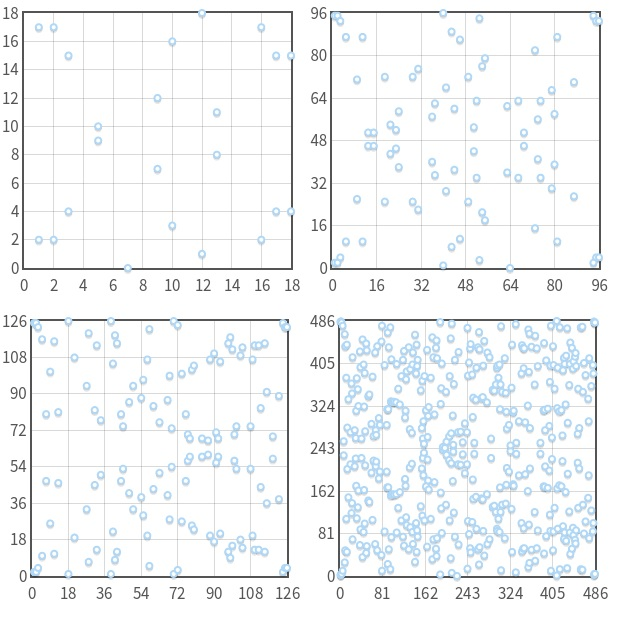
\includegraphics[width=9cm]{Figures/EC_ex.jpg}
	\caption{Points on the Elliptic Curve $y^2=x^3-7x+10 \; \textrm{mod} \ p$, with $p=19,97,127,487$ }
	\label{fig:EC_ex}
\end{figure}

\subsection{Symmetry}
The elliptic curve has an important property: the line $y=p/2$ is an axis of symmetry for the curve.
\\ \\
This can be shown, by proving that the point $P(x,y)$ belongs to the Elliptic Curve ($EC$) if and only if the point $Q(x,p-y)$ belongs to the curve too:
\begin{equation*}
P(x,y) \in EC \iff Q(x,p-y) \in EC.
\end{equation*}
\textit{Proof}:
\\ \\
First analyze the implication in the right direction: ($\implies $).
\\ \\
From Equation (\ref{GeneralECmodp}) and from the hypothesis we have that:
\begin{equation*}
P(x,y) \in EC \implies y^2=x^3+ax+b \quad \textrm{mod} \ p,
\end{equation*}
but we know also that: 
\begin{equation*}
Q(x,p-y) \in EC \iff (p-y)^2=x^3+ax+b \quad \textrm{mod} \ p.
\end{equation*}
From the moment that the right hand side of both the equations are equal, we only need to prove that:
\begin{equation*}
(p-y)^2=y^2 \quad \textrm{mod} \ p.
\end{equation*}
This is true, indeed:
\begin{align*}
(p-y)^2 & = p^2 -2py + y^2 &  \textrm{mod} \ p \\
& = p\cdot(p -2y) + y^2 &  \textrm{mod} \ p \\
& = 0+y^2 &  \textrm{mod} \ p \\
& = y^2 &  \textrm{mod} \ p
\end{align*}
This is due to the fact that 
\begin{equation*}
p\cdot k =0 \quad \textrm{mod} \ p \qquad \forall k\in \mathbb{N}.
\end{equation*}
The other implication ($\impliedby$) is almost the same and it follows the same logic.
\begin{flushright}
	\textit{c.v.d.}
\end{flushright}
Once shown the symmetry property, it can be useful to denote the point $P(x,y)$ as the opposite of $Q(x,p-y)$:
\begin{equation*}
P=-Q \implies P+Q=0,
\end{equation*}
where the $+$ operator between two points in the EC will be explained below and the $0$ in this contest is the \textit{point at infinity}.

\subsection{Point addition}
Once defined a point on the elliptic curve, let's introduce the addition between two points on this finite field.
\\ \\
We need to change our definition of addition in order to make it works in $\mathbb{F}_p$. In this framework, we claim that if some points are aligned over the finite field $\mathbb{F}_p$, then they have zero-sum.
\\ \\
So $P+Q=R$ if and only if $P$, $Q$ and $-R$ are aligned, in the sense shown in Figure \ref{fig:EC_aligned}
\begin{figure}[ht!]
	\centering
	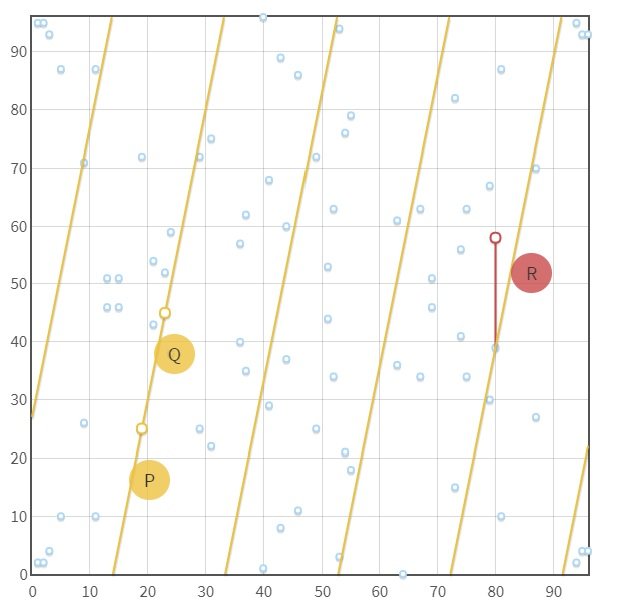
\includegraphics[width=9cm]{Figures/EC_aligned.jpg}
	\caption{Elliptic Curve $y^2=x^3-7x+10 \; \textrm{mod} \ 97$}
	\label{fig:EC_aligned}
\end{figure}

\begin{flushleft}
	After defined when points in the EC have zero-sum, it is possible to calculate the equations for point addition:
\end{flushleft}
Suppose that \textit{A} and \textit{B} belong to the Elliptic Curve.

\begin{center}
	$ A=(x_1,y_1) \quad B=(x_2,y_2)$.
\end{center}
Let's define $ A+B :=(x_3,y_3) $ 
\\ \\
When $x_1=x_2$ but $y_1 \neq y_2$, it is the case in which $A$ and $B$ are symmetric point and so the sum is a particular point, called \textit{point at infinity}: 
\begin{equation*}
A+B=0=	(inf,inf) .
\end{equation*}
In all the other cases we have:



\begin{center} 
	$s=\begin{cases} \dfrac{y_2-y_1}{x_2-x_1}, & \mbox{if } x_1\neq x_2, \; y_1\neq y_2 \;\rightarrow \; \text{point addition},\\ \\ \dfrac{3x_1^2+a}{2y_1}, & \mbox{if } x_1= x_2, \; y_1= y_2 \;\rightarrow \; \text{point doubling}, \end{cases}$
\end{center}
where $s$ is a dummy variable, used to compute $x_3$ and $y_3$. It can be computed in two different way: if we are performing a "real" point addition, when $A\neq B$ or if we are looking for the double of a point, when $A= B$.
\begin{center} 
	$ x_3=s^2-x_1-x_2  \quad$ mod $p$,\\
	$y_3=s(x_1-x_3)-y_1  \quad$mod $p$.
\end{center}
Once we have $s$ the value $x_3$ and $y_3$ are obtained following this simple formula.


\subsection{Scalar multiplication}
Once defined the addition, any multiplication between a scalar and a point on the elliptic curve can be defined as:
\begin{center} 
	$ nP=\underbrace{
		P+P+\cdot \cdot \cdot+P
	}_{n\text{ times}}$.
\end{center}
When $n$ is a very large number can be difficult or even infeasible to compute $nP$ in this way, but we can use the \textit{double and add algorithm} in order to perform multiplication in $\mathcal{O}(\log{}n)$ steps. Let's see an example:
\\ \\
Suppose that we need to compute $53 \cdot P$ where $P$ is a point on the EC:
\begin{equation*}
53 \cdot P = 110101_{base\, 2} \cdot P = 2^{5}\cdot P + 2^{4}\cdot P + 2^{2}\cdot P + P
\end{equation*}
Computing the common sub-terms only once we obtain a total of 5 doubling and 3 addition operations, much less of 52 addition operations. This algorithm is even more efficient if the scalar is a very large number.

\subsection{Discrete Logarithm Problem}
Once we have described the multiplication between a scalar and a point, let's see if it is possible to make the inverse operation. Let's suppose that:
\begin{equation*}
Q = n \cdot P,
\end{equation*}
where $Q$ and $P$ are points on the EC and $n$ is a scalar number. 
\\ \\ 
Let's suppose to know $Q$ and $P$. With these information it exists only one possible $n \in \mathbb{N}$, such that $0<n<p$ and that the equation above holds true. Even so this number $n$ is infeasible to find for large value of $p$.
\\ \\
This is due to the fact that there is not an efficient algorithm that is able to compute $n$ given $P$ and $Q$. The only way to find $n$ is by trying. As already mentioned, this could become infeasible if the number of value that $n$ can assume ($p-1$) is too large.

\subsection{Group order}
An elliptic curve defined over a finite field is a group and so it has a finite number of points. This number is called \textit{order} of the group.
\\ \\
If $p$ is a very large number, it is impossible to count all the points in that field, but there is an algorithm that allows to calculate the \textit{order} of a group in a fast and efficient way: \textit{Schoof's algorithm}.
\\ \\
Let's consider a generic point $G$, we have:
\begin{center} 
	$ nG+mG=\underbrace{
		G+\cdot \cdot \cdot+G
	}_{n\text{ times}}+
	\underbrace{
		G+\cdot \cdot \cdot+G
	}_{m\text{ times}}=
	\underbrace{
		G+\cdot \cdot \cdot+G
	}_{n+m\text{ times}} = 
	(n+m)G$.
\end{center}
So multiples of $G$ are closed under addition and this is enough to prove that the set of the multiples of $G$ is a cyclic subgroup of the group formed by the elliptic curve.
\\ \\
The point $G$ is called \textbf{generator} of the cyclic subgroup.

\begin{remark}
	The order of the subgroup generated by $G$ is linked to the order of the elliptic curve by Lagrange's theorem, which states that the order of a subgroup is a divisor of the order of the parent group.
\end{remark}

\begin{remark}
	If the order of the group is a prime number, all the points belonging to the EC generate a subgroup with the same order of the group or with order 1.
\end{remark}
All these preliminary information are needed in order to introduce the private-public key cryptography used by Bitcoin.





\subsection{Bitcoin private-public key cryptography}

Bitcoin [\cite{11}] uses a specific Elliptic Curve defined over the finite field of the natural numbers, where $a=0$ and $b=7$.\\ \\
The Equation (\ref{GeneralEC}) becomes:
\begin{equation}\label{BitcoinEC}
y^2=x^3+7 \quad \textrm{mod} \ p,
\end{equation}
where the \textit{mod p} (modulo prime number) indicates that this curve is over a finite field of prime order $p=2^{256}-2^{32}-2^9-2^8-2^7-2^6-2^4-1$.
\\ \\
The \textit{order} of this Elliptic Curve is a very large prime number, close to $2^{256}$, but smaller then $p$. \\ \\
Let's consider a particular point $G$, called generator, expressed in hexadecimal digits:
\begin{center} 
	$ x=79BE667E F9DCBBAC 55A06295 CE870B07 029BFCDB 2DCE28D9 59F2815B 16F81798$\\
	$y=483ADA77 26A3C465 5DA4FBFC 0E1108A8 FD17B448 A6855419 9C47D08F FB10D4B8$
\end{center}
From the moment that the order of the group is a prime number, the order of any subgroup is equal to the order of the entire group. In particular, the order of the subgroup generated by $G$ is equal to \textit{order}.
\\ \\
We have now all the elements necessary to define the private and the public key.
\begin{definition}
	A private key is a number chosen in the range between 1 and order.
\end{definition}

\begin{definition}
	A public key $W$ is a point in the Bitcoin EC, derived from a private key $k$ in the following way: \\
	\begin{equation}
	W=k\cdot G,
	\end{equation}
	where the multiplication between k and G is defined in the previous chapter.
\end{definition}
This is a \textit{one way} function: it is simple to compute the scalar multiplication, knowing the private key, but it is infeasible to do the opposite.
\begin{remark}
	It is infeasible to calculate a private key knowing the public key.
\end{remark}
The purpose of having defined the private and public keys is to use them to cryptographically sign a message. It is not the scope of this thesis explain how a message is signed, but it is at least necessary to know the principal properties of a signed message.
\\ \\
Let's suppose to have a message that is needed to be signed, in Bitcoin this message is usually a \textit{transaction}.

\begin{itemize}
	\item A message is signed using a \textbf{private key}.
	\item Knowing the \textbf{public key} associated with the private key that signs the message, it is possible to verify that the message is signed using the corresponding private key (without knowing it).
\end{itemize}
For this reason the keys are called private and public, the former is suppose to be kept \textbf{secret} because it is able to sign a message, instead the latter is suppose to be \textbf{shared}, in order to let everyone else knows that who signs the message is in possession of the corresponding private key.






	% Chapter 1

\chapter{Wallet} % Main chapter title

\label{wallet} % For referencing the chapter elsewhere, use \ref{Chapter1}

%----------------------------------------------------------------------------------------

% Define some commands to keep the formatting separated from the content 
%\newcommand{\keyword}[1]{\textbf{#1}}
%\newcommand{\tabhead}[1]{\textbf{#1}}
%\newcommand{\code}[1]{\texttt{#1}}
%\newcommand{\file}[1]{\texttt{\bfseries#1}}
%\newcommand{\option}[1]{\texttt{\itshape#1}}

%----------------------------------------------------------------------------------------


A Bitcoin wallet is a structure used to store keys. \\ \\
There are different type of wallet:
\begin{itemize}
	\item Nondeterministic (\textit{random}) Wallet
	\item Deterministic Wallet
\end{itemize}

\begin{remark}
	Bitcoin wallets contains keys, not coins. Coins are in the Blockchain.
\end{remark}

\section{Nondeterministic (\textit{random}) Wallet}
A nondeterministic wallet is the simplest type of wallet. Each Key is randomly and independently generated.

\begin{enumerate}[label=(\roman*)]
	\item Consider a \textit{Discrete Uniform Random Variable}
	\begin{equation*}
		X\sim \mathcal{U}(S)
	\end{equation*}
	Where $S$ is the finite set of natural number in the range from $1$ to $order$.
	\item Take some realizations $k_1,k_2...k_n$ of $X$ using enough entropy to make these numbesr (\textit{private keys}) impossible to guess.
	\begin{equation*}
		k_1=X(\omega_1) \quad  k_2=X(\omega_2) \quad ... \quad k_n=X(\omega_n)
	\end{equation*}
	\item Go back to point (i) every time new \textit{private keys} are needed.
\end{enumerate}
With this procedure it is impossible to compute the \textit{public key} without having already the \textit{private key}.

\subsubsection{Pros and Cons}
Let's focus on the good and bad aspects of this wallet.

\begin{center}
	\begin{tabular}{ |p{6cm}|p{6cm}|  }
	\hline
	\multicolumn{2}{|c|}{\textbf{\textit{Random Wallet}}} \\
	\hline \hline 
	\begin{center}
		\textbf{Pros}
	\end{center}&\begin{center}
		\textbf{Cons}
	\end{center}\\
	\hline
	\begin{itemize}
		\item Easy to implement
	\end{itemize} &
	\begin{itemize}
		\item Difficult to find \underline{real} new entropy for every new \textit{private key}.
		\item Every time new \textit{private keys} are needed, you need to make new back up.
		\item Difficult to store or back up in a \textit{non digital way}. Awkward to write it down all yours keys on a paper.
	\end{itemize}\\
	\hline
\end{tabular}
\end{center}

The use of \textit{random wallet} is strongly discouraged for anything other than simple test. There are no good reason to use it.

\section{Deterministic Wallets}
A deterministic wallet is a more sophisticated one, in which every key is generated from a common "\textit{seed}". This means that knowing the \textit{seed} means also to know all the keys in the wallet.\\ \\
There are different types of deterministic wallets, in this text we will analyze three main types:
\begin{itemize}
	\item Deterministic Wallet \textit{type 1}
	\item Deterministic Wallet \textit{type 2}
	\item Deterministic Wallet \textit{type 3}
\end{itemize}
These wallet are in increasing order of complexity.

\subsection{Deterministic Wallet \textit{type-1}}
The Deterministic Wallet \textit{type-1} is one of the simplest Wallet among the deterministic ones. Each key is generated adding a number in a sequential order to the \textit{seed} and then computing an \textit{hash} function such as the \textbf{SHA256} function.
\\ \\
Let's see how to generate the $n^{th}$ private key:

\begin{enumerate}[label=(\roman*)]
	\item Generate a \textit{seed} (only once), a random number from a \textit{Discrete Uniform Random Variable}
	\begin{equation*}
	seed=X(\omega) \qquad X\sim \mathcal{U}(S)
	\end{equation*}
	Where $S$ is the finite set of natural number in the range from $1$ to $order$.
	\item Consider the numbers $seed$ and $n$ as strings and concatenate $n$ to $seed$, obtaining a $value$
	\begin{equation*}
	value=seed|n
	\end{equation*}
	\item Compute the SHA256 function to $value$ and obtain the $n^{th}$ \textit{private key}.
	\item Go back to point (ii) every time new \textit{private keys} are needed with $n=n+1$. 
\end{enumerate}
With this procedure it is impossible to compute the \textit{public key} without having already computed the \textit{private key}.

\subsubsection{Pros and Cons}
Let's focus on the good and bad aspects of this wallet.

\begin{center}
	\begin{tabular}{ |p{6cm}|p{6cm}|  }
		\hline
		\multicolumn{2}{|c|}{\textbf{\textit{Deterministic Wallet type-1}}} \\
		\hline \hline 
		\begin{center}
			\textbf{Pros}
		\end{center}&\begin{center}
			\textbf{Cons}
		\end{center}\\
		\hline
		\begin{itemize}
			\item In order to make a back up of the entire wallet it is needed to store the \textit{seed} only. All \textit{private keys} can be derived from it.
			\item A single back up is needed.
			\item The \textit{seed} can be stored easily also in a \textit{non digital way}, in a paper for example.
		\end{itemize} &
		\begin{itemize}
			\item Every time new \textit{public keys} are needed, you need to use the \textit{seed}, to compute new \textit{private keys} and then derive the \textit{public} ones. This could compromise the entire wallet, if the \textit{seed} is used in a non safe environment.
			\item There is only a \textit{key} sequence. No way to distinguish the "purpose" of each \textit{private key}.
		\end{itemize}\\
		\hline
	\end{tabular}
\end{center}
The use of this type of wallet is not recommended for everyday use, but it could be used to store Bitcoin in a safe place: \textit{cold wallet}. 

\subsection{Deterministic Wallet \textit{type-2}}
The Deterministic Wallet \textit{type-2} is more sophisticated. Each \textit{private key} is generated in such a way that it is possible to compute the respective \textit{public key} without knowing the \textit{private}.
\\ \\
First let's introduce the necessary ingredients:
\begin{itemize}[label=$\diamond$]
	\item \textbf{Master private key} ($mp$): a random number, generated from a \textit{Discrete Uniform Random Variable}
	\begin{equation*}
	mp=X(\omega) \qquad X\sim \mathcal{U}(S)
	\end{equation*}
	Where $S$ is the finite set of natural number in the range from $1$ to $order$. \\ The master private key must be take \underline{secret}.
	\item \textbf{Master public key} ($MP$): a point on the EC, obtained from the $mp$:
	\begin{equation*}
	MP=mp\cdot G
	\end{equation*}
	Where $G$ is the \textit{generator}.\\ This point can be consider \underline{non-secret}.
	\item \textbf{Public random number} ($r$): a random number, generated from a \textit{Discrete Uniform Random Variable}
	\begin{equation*}
	r=X(\omega) \qquad X\sim \mathcal{U}(S)
	\end{equation*}
	This number can be consider \underline{non-secret}.
\end{itemize}
Let's see how to generate the $n^{th}$ private key: $p_n$

\begin{enumerate}[label=(\roman*)]
	\item Compute the SHA256 function to the concatenation of $r$ with $n$, considered as string:
	\begin{equation*}
	h_{n|r}=SHA256 (n|r)
	\end{equation*}
	$h_{n|r}$ can be consider \underline{non-secret}, from the moment that it is derived from non secret information.
	\item Compute the $n^{th}$ \textit{private key} adding $mp$ to $h_{n|r}$:
	\begin{equation*}
	p_n=mp+h_{n|r} \qquad \mod (order)
	\end{equation*}
\end{enumerate}
In order to obtain the corresponding \textit{public key} $P_n$, it is possible to compute the standard multiplication:
\begin{equation*}
P_n=p_n \cdot G
\end{equation*}
It is also possible to compute $P_n$ without knowing $p_n$, using only non-secret information: $h_{n|r}$ and $MP$.
\begin{enumerate}[label=(\roman*)]
	\item Compute $V$:
	\begin{equation*}
	V=h_{n|r} \cdot G
	\end{equation*}
	$V$ can be see as the \textit{public key} of $h_{n|r}$ and can be consider \underline{non-secret}.
	\item Add $MP$ to $V$:
	\begin{equation*}
	P_n=MP+V
	\end{equation*}
	Where the sum in this contest is the one defined between two point in the EC.
\end{enumerate}
It is easy to prove that $P_n$ can be computed in these two way:
\begin{equation*} \label{eq1}
\begin{split}
P_n & = p_n \cdot G \\
& = (mp+h_{n|r}) \cdot G \\
& = (mp \cdot G) + (h_{n|r}\cdot G) \\
& = MP + V
\end{split}
\end{equation*}

\subsubsection{Pros and Cons}
Let's focus on the good and bad aspects of this wallet.

\begin{center}
	\begin{tabular}{ |p{6cm}|p{6cm}|  }
		\hline
		\multicolumn{2}{|c|}{\textbf{\textit{Deterministic Wallet type-2}}} \\
		\hline \hline 
		\begin{center}
			\textbf{Pros}
		\end{center}&\begin{center}
			\textbf{Cons}
		\end{center}\\
		\hline
		\begin{itemize}
			\item In order to make a back up of the entire wallet it is needed to store the \textit{master private key} and the random number $r$. All \textit{private keys} can be derived from them.
			\item A single back up is needed.
			\item The \textit{master private key} can be stored easily also in a \textit{non digital way}, in a paper for example.
			\item It is possible to derive a new \textit{public key} using only non-secret information, with the procedure above.
		\end{itemize} &
		\begin{itemize}
			\item There is only a \textit{key} sequence. No way to distinguish the "purpose" of each \textit{private key}.
		\end{itemize}\\
		\hline
	\end{tabular}
\end{center}
The \textit{type-2 deterministic wallet} it is an improvement of the \textit{type-1} because it has the same benefits (except for the need to back up two number instead of only one), but with a great advantage: it is possible to generate new addresses also in a non safe environment, having only $r$ and $MP$. \\
A thief can only steal your privacy, because if $MP$ and $r$ are stolen, he is not able to make any Bitcoin transactions from your wallet, but he can see all the previous transactions and the total amount of Bitcoin stored in the wallet.

\subsection{Deterministic Wallet \textit{type-3}}
Deterministic Wallet \textit{type-3} is the most elaborate among the ones considered. Starting from a \textit{seed} it is possible to obtain different \textit{keys} in a hierarchical way, with a structure similar to a tree. \\ \\
Let's see roughly how an this Wallet works:

\begin{enumerate}[label=(\roman*)]
	\item Generate a \textit{seed}, a random number from a \textit{Discrete Uniform Random Variable}, unique for each wallet.
	\begin{equation*}
	seed=X(\omega) \qquad X\sim \mathcal{U}(S)
	\end{equation*}
	Where $S$ is a finite set of natural number.
	\item Generate a \textit{master private key} from the \textit{seed}, using a stretching function: PBKDF2.
	\item From this \textit{master private key} it is possible to generate $2^{8}$ \textit{private key} using a irreversible function: HASH512
	\item Everyone of this \textit{private key} "children" can derive $2^{8}$ \textit{private key} and all of these "grandchildren" can derive as many.
\end{enumerate}

This procedure can produce a huge number of keys. They seem independent from an outside point of view: it is impossible to guess that two private-public key are derived from the same \textit{seed}.
\\ \\ 
This particular type of Wallet is commonly known as \textbf{Hierarchical Deterministic Wallet}, one of the most used and widespread.
\\ \\
In the next chapter we will see in detail how it works.

	% Chapter 1

\chapter{Hierarchical Deterministic Wallet} % Main chapter title

\label{hd wallet} % For referencing the chapter elsewhere, use \ref{Chapter1}

%----------------------------------------------------------------------------------------

% Define some commands to keep the formatting separated from the content 
%\newcommand{\keyword}[1]{\textbf{#1}}
%\newcommand{\tabhead}[1]{\textbf{#1}}
%\newcommand{\code}[1]{\texttt{#1}}
%\newcommand{\file}[1]{\texttt{\bfseries#1}}
%\newcommand{\option}[1]{\texttt{\itshape#1}}

%----------------------------------------------------------------------------------------

In this chapter we will see how an HD wallet works.
\\ \\
\section{Elements}
Let's focus on the main elements of the Wallet:
\begin{itemize}[label=$\diamond$]
	\item Seed
	\item Extended keys
\end{itemize}

\subsection{Seed}
The entire Wallet is based on a \textit{seed}.
\\ \\
It is a number taken from a \textit{Discrete Uniform Random Variable}
\begin{equation*}
seed=X(\omega) \qquad X\sim \mathcal{U}(S)
\end{equation*}
Where $S$ is the finite set of natural number in the range from $1$ to an arbitrary value.\\ Obviously the greater the set from which the number can be extracted, the better it is for the security of the seed itself.
\\ \\
This is an example of seed expressed in hexadecimal format: \\
\textit{seed}=fffcf9f6f3f0edeae7e4e1dedbd8d5d2cfccc9c6c3c0bdbab7b4b1aeaba8a5a29f9c999 \\ 693908d8a8784817e7b7875726f6c696663605d5a5754514e4b484542 

\subsection{Extended Key}
An Extended Key is a sequence of bytes, encoded in base58. It contains all the information necessary for the derivation. When the derivation is made for the first time from the seed, the extended key is called master key.\\ \\
Once it is decoded we will obtain exactly 78 bytes, with a specific meaning and order:
\begin{itemize}[label=$\circledast$]
	\item 4 bytes are used to specified the \textbf{version}.
	\item 1 byte is used to specified the \textbf{depth} in the hierarchical tree: the extended key derived directly from the seed has $depth=0$, its first children have $depth=1$, grandchildren have $depth=2$ and so on.
	\item 4 bytes are used for the \textbf{fingerprint}. It is a unique value that identify the parent. Compute the HASH160 function on the "parent" public key in a compressed form and then take the first 4 bytes, this is the fingerprint of the child:
	\begin{equation*}
	fingerprint=HASH160(\text{parent public key})[0:4]
	\end{equation*}
	Where $[0:4]$ is a python notation.\\
	For the master key the fingerprint is formed by 4 zeros bytes: $fingerprint=0000000000$
	\item 4 bytes are used to specified the \textbf{index} of the child. \\
	For the master key the index is formed by 4 zeros bytes: $index=0000000000$
	\item 32 bytes are used for the \textbf{chain code}. The chain code is used in order to introduce a sort of entropy in the children generation. We will see below how it works.
	\item 33 bytes are used for the \textbf{key}. It can be \textit{private} or \textit{public}. \\ Public key is expressed in compact form, so the first byte is always $02$ or $03$. The first byte of the private key is always $00$ in order to distinguish the key from the public one.\\
\end{itemize}
An extended key is called \textbf{Extended Private Key} if the lasts 33 bytes are used to specify the private key; it is called \textbf{Extended Public Key} if they are used to specify the public key.
\\ \\
For the Bitcoin mainnet it is used for the \textbf{version}: $0x0488ADE4$ for an extended private key, $0x0488B21E$ for an extended public key. When this bytes are encoded in base58, they returns \textit{xprv} and \textit{xpub} respectively.

\begin{remark}
	Obviously it is possible to calculate the extended public key starting from the extended private key, but it is infeasible to do the opposite. The only difference between the two extended keys are the \textbf{key bytes} and the \textbf{version bytes}, all the others elements remain the same.
\end{remark}

\section{From SEED to Master Private Key}
In this section we will see in detail how it is possible to switch from a \textit{seed} to a \textit{master private key}. \\ \\
First of all we need to convert the seed into a string of bytes, where the most significant bytes come first (big endian). In order to do so, we need to know how much long we want the string of bytes. \\ \\
Let's see a practical example:
\begin{equation*}
\begin{split}
&byte\_string_1=00\; 00\; 00 \; 01 \\
&byte\_string_2=00\; 00\; 01 \\
&byte\_string_3=00\; 01 \\
&byte\_string_4=01
\end{split}
\end{equation*}
These $4$ byte strings are obtained from the same seed: $seed=1$ and the only different is the length of the string.
\begin{remark}
	Different length of string produce different master private key, even if the seed is the same number.
\end{remark}
In python:
\begin{lstlisting}[language=Python]
byte_string = seed.to_bytes(seed_bytes, 'big')
\end{lstlisting}
Where $seed$ is a \textit{int}, \textit{seed\_bytes} is the number of bytes that the \textit{byte\_string} should have. \\ \\
It is essential to specify the length of the byte string, otherwise there will be obtained different wallets. \\ \\
Once we obtain a string of bytes, we will compute the HMAC algorithm. The hash function used for HMAC is the SHA512 and the \textit{key} is a particular string of bytes: \textit{b"Bitcoin seed"}. In python the implementation is the follow:

\begin{lstlisting}[language=Python]
from hashlib import sha512
from hmac import HMAC

hashValue = HMAC(b"Bitcoin seed", byte_string, sha512).digest()
\end{lstlisting}
Where \textit{.digest()} is used in order to return a string of bytes.
\\ \\
Now we have obtained an \textit{hashValue} of $512$ bits, so $64$ bytes. Consider the firsts $32$ bytes as the master private key and the next $32$ bytes as the master chain code. A python implementation is the follow:

\begin{lstlisting}[language=Python]
private_key_bytes = hashValue[0:32]
chain_code_bytes = hashValue[32:64]
\end{lstlisting}
\begin{flushleft}
	Now we have two byte strings, one for the master private key and the other for the master chain code.
\end{flushleft}
It is important to remember that a private key must be in the range between $1$ and $order$, so the byte string for the private key should be converted in \textit{int} and then take the \textit{mod order}. In python we have:

\begin{lstlisting}[language=Python]
private_key = int(private_key_bytes.hex(), 16) % order
\end{lstlisting}
\begin{flushleft}
	Finally we will concatenate all the informations obtained in order to form a Master Extended Private Key (in bytes format):
\end{flushleft}

\begin{itemize}
	\item vbytes = $b'\backslash x04\backslash x88\backslash xAD\backslash xE4'$
	\item depth = $b'\backslash x00'$
	\item fingerprint = $b'\backslash x00\backslash x00\backslash x00\backslash x00'$
	\item index = $b'\backslash x00\backslash x00\backslash x00\backslash x00'$
	\item chain code is the one previously computed
	\item private key = $b'\backslash x00'$ $+$ private key in bytes format, previously computed.
\end{itemize}
Then the Master Extended Private Key is formed by concatenation:

\begin{lstlisting}[language=Python]
xkey = vbytes + depth + fingerprint + index + chain_code + key
\end{lstlisting}
\begin{flushleft}
	In order to make it readable, a base58 encode is performed.
\end{flushleft}
This is an example of Master Extended Private Key: \\
xprv9s21ZrQH143K3wEaiSJZ8jYCuZF1oJoXHiwFcx2WwXqQHD4ZLdyEAFZ22M4 BmQT82HRbWssLArj53YDQTj6vSN4iH6nTiSQ61C5CckxUtDq

\begin{remark}
	The SHA512 is an irreversible function, so it is infeasible to obtained the seed, knowing the Extended Key. (It is also useless because with the master key you can derive all the keys in the wallet).
\end{remark}

\begin{flushleft}
	Graphically these operation can be shown in figure \ref{fig:From seed to master private key}
\end{flushleft}

\begin{figure}[ht!]
	\centering
	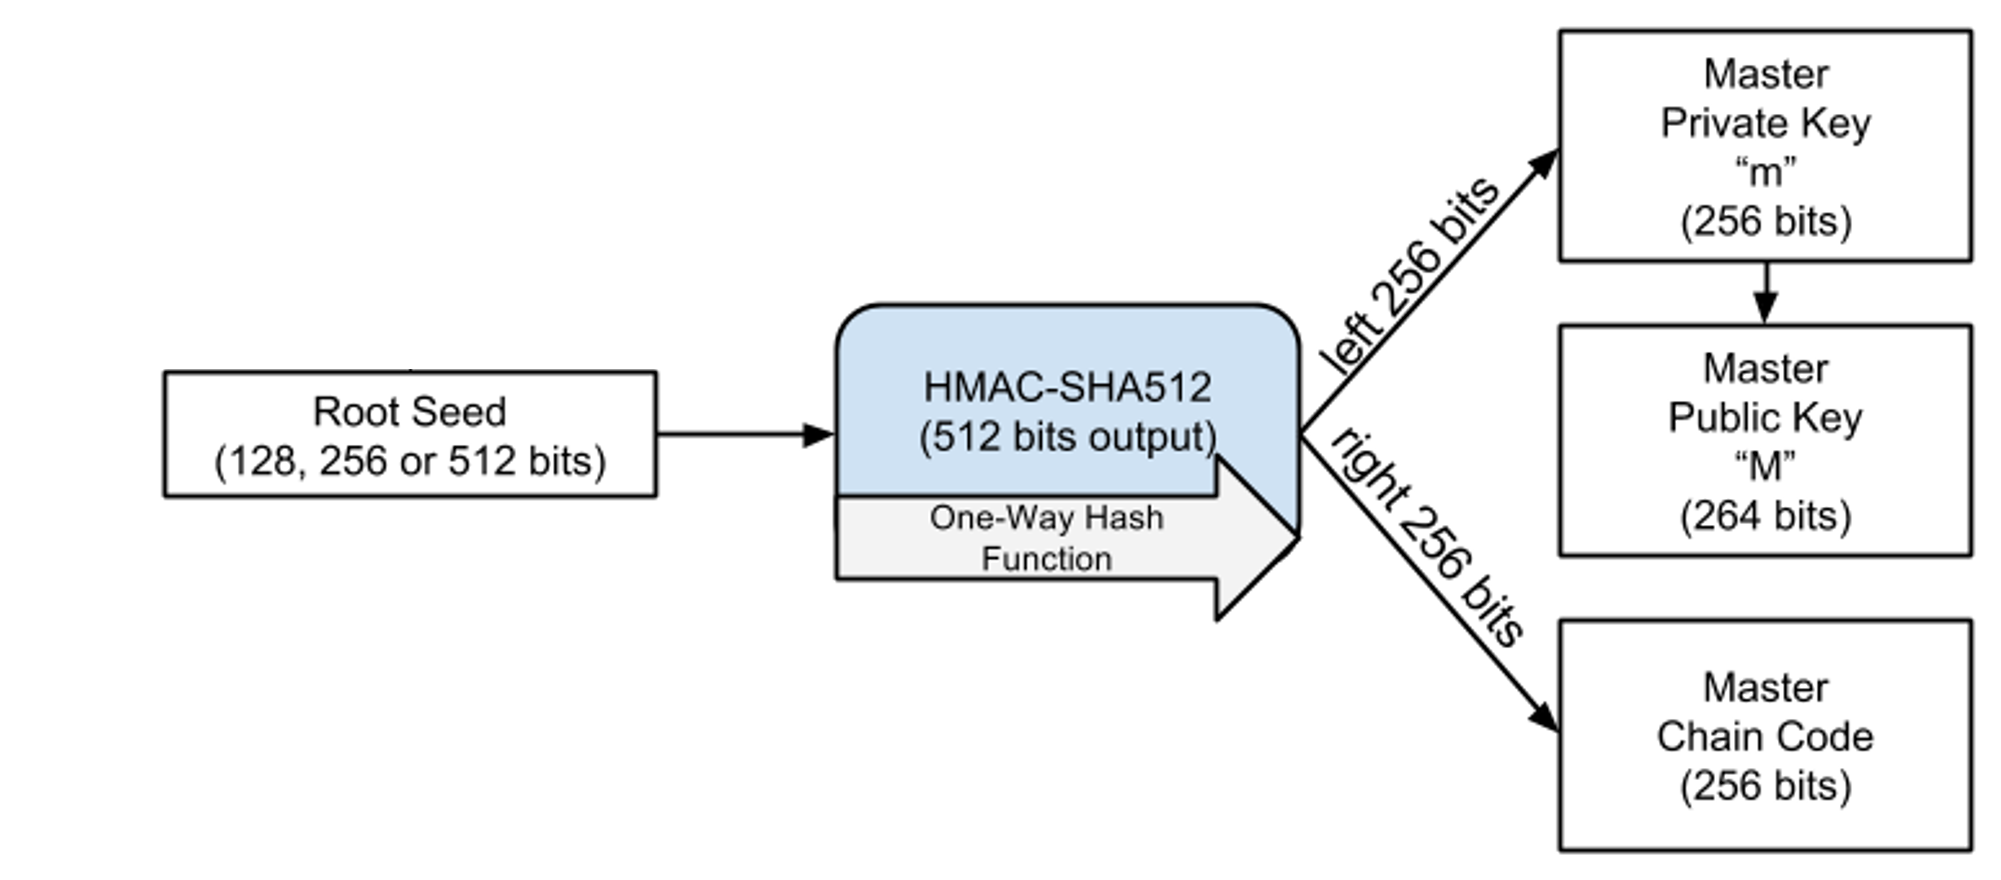
\includegraphics[width=13cm]{Figures/seed_to_xprv.png}
	\caption{From seed to master private key}
	\label{fig:From seed to master private key}
\end{figure}


\section{Child Key derivation}
From any extended private key it is possible to obtain different child keys. There are two method used in order to do so:
\begin{itemize}
	\item Normal
	\item Hardened
\end{itemize}
Both methods have some advantage and disadvantage that we will discuss later. For every situation it is essential to use the method that best fit.
\\ \\
For both the method the derivation starts from a Extended Private Key. From this key some essential information are necessary:
\begin{itemize}[label=$\star$]
	\item Chain code
	\item Private key
\end{itemize}
It is also required a number, used in order to specify the \textbf{index} of the child. This number should be in the range between $0$ and $4294967295$. This is due to the fact that in any Extended Key there are 4 bytes used to specify the index of the child:
\begin{equation*}
	max \; index=(FF\;FF\;FF\;FF)_{16} = (4294967295)_{10}
\end{equation*}
In fact it is possible to generate even a greater number of children from the same parent, but it would not be possible to write the corresponding Extended Key in the format described above.


\subsection{Normal derivation}

As already mentioned we need only 3 ingredient in order to derive a key. Let's see how we can combine them together in order to obtain a new key (and chain code). \\ \\
First we need to compute the Parent Public Key $P$. This is obtained from the usual scalar multiplication of an EC point (the Generator $G$) with the Parent Private Key $p$:

\begin{equation*}
P=p\cdot G
\end{equation*}
Consider only the compress form of $P$ and convert this value into a byte string, obtaining 33 bytes.
\\ \\
Concatenate this 33 byte string to the 4 byte string representing the index number:

\begin{equation*}
msg = compressed \; public\;key \;|\; index
\end{equation*}
$msg$ is a string of $37$ bytes. \\ \\
Apply the HMAC algorithm with the following input:

\begin{itemize}[label=$\odot$]
	\item \textbf{Hash function}: SHA512
	\item \textbf{Key}: chain code
	\item \textbf{Message}: $msg$
\end{itemize}
The Python code is the follow:
\begin{lstlisting}[language=Python]
from hmac import HMAC
from hashlib import sha512

msg=parent_public_key + index
hashValue = HMAC(parent_chain_code, msg, sha512).digest()
\end{lstlisting}
\begin{flushleft}
	The result is a string of 64 bytes: \textit{hashValue}.
\end{flushleft}
Split this string of bytes in two: the last 32 are the child chain code. Take the first 32 bytes, convert them into an integer number and sum it to the parent private key (mod \textit{order}), obtaining the child private key.\\ \\
This is the python code:

\begin{lstlisting}[language=Python]
child_chain_code = hashValue[32:]
q = int(hashValue[:32].hex(), 16)
child_private_key = (q + parent_private_key) % order
\end{lstlisting}

\begin{flushleft}
	Graphically these operation can be shown in figure \ref{fig:normal_derivation}
\end{flushleft}

\begin{figure}[ht!]
	\centering
	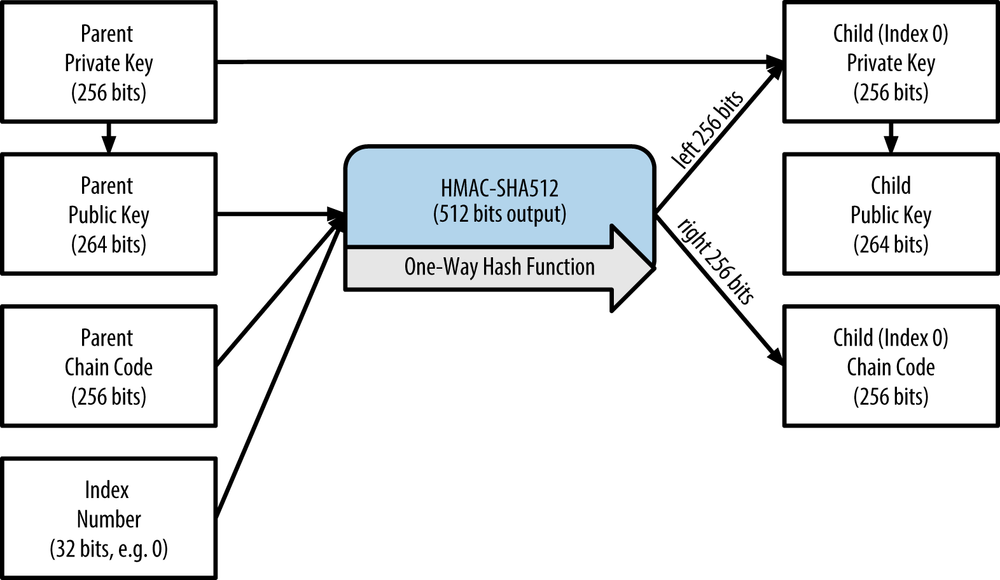
\includegraphics[width=15cm]{Figures/normal_derivation.png}
	\caption{Normal Derivation }
	\label{fig:normal_derivation}
\end{figure}


\subsection{Hardened derivation}
This method is similar to the previous one, the only difference is that as input of the \textit{hash} function the private key is used instead of the public one. \\ \\
Concatenate the 33 bytes of parent private key, considering also the $00$ byte, with the 4 byte string representing the index number:

\begin{equation*}
msg = 00 \;|\; private\;key \;|\; index
\end{equation*}
$msg$ is a string of $37$ bytes. \\ \\
Apply the HMAC algorithm with the following input:

\begin{itemize}[label=$\odot$]
	\item \textbf{Hash function}: SHA512
	\item \textbf{Key}: chain code
	\item \textbf{Message}: $msg$
\end{itemize}
The Python code is the follow:
\begin{lstlisting}[language=Python]
from hmac import HMAC
from hashlib import sha512

msg=parent_private_key + index
hashValue = HMAC(parent_chain_code, msg, sha512).digest()
\end{lstlisting}
\begin{flushleft}
	The result is a string of 64 bytes: \textit{hashValue}. In this code the $parent\_private\_key$ already has the first $00$ byte, because it is taken directly from the parent extended private key.
\end{flushleft}
Split this string of bytes in two (in the same way as the normal method): the last 32 are the child chain code. Take the first 32 bytes, convert them into an integer number and sum it to the parent private key (mod \textit{order}), obtaining the child private key.\\ \\
This is the python code:

\begin{lstlisting}[language=Python]
child_chain_code = hashValue[32:]
q = int(hashValue[:32].hex(), 16)
child_private_key = (q + parent_private_key) % order
\end{lstlisting}


\begin{flushleft}
	Graphically these operation can be shown in figure \ref{fig:hardened_derivation}
\end{flushleft}

\begin{figure}[ht!]
	\centering
	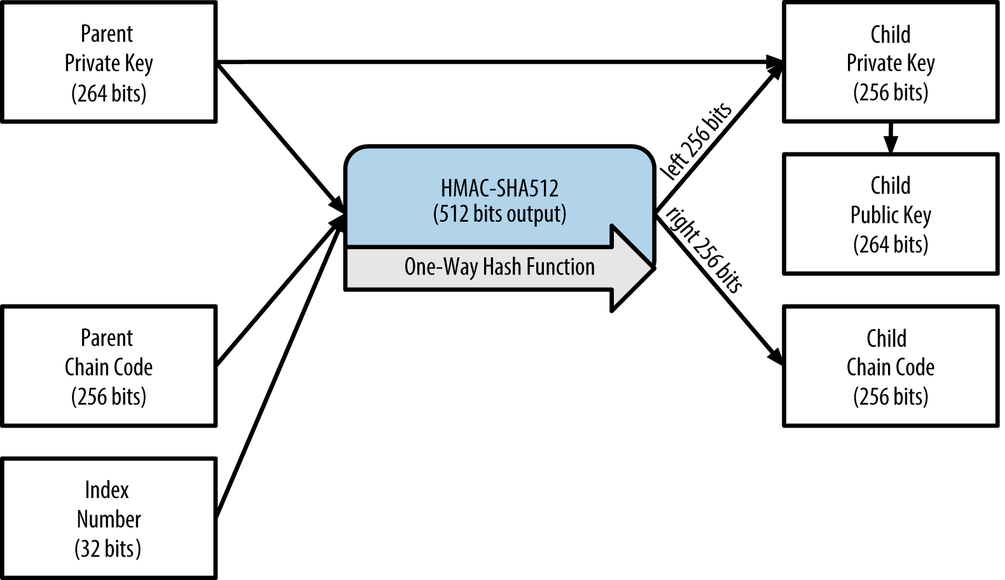
\includegraphics[width=15cm]{Figures/hardened_derivation.png}
	\caption{Hardened Derivation }
	\label{fig:hardened_derivation}
\end{figure}


\section{Special derivation}
Using a \textit{normal derivation} it is possible to derive the extended public key, starting only from the extended public key of the parent.

\subsection{Public derivation}

The only essential elements are the ones contained in the extended public key, in particular:

\begin{itemize}
	\item Public key $P_{parent}$
	\item Chain code
	\item Index
\end{itemize}

As shown for the normal derivation starting from the extended private key, we have all the input elements for the hash algorithm:
\\ \\
Concatenate the 33 byte string of the public key to the 4 byte string representing the index number:

\begin{equation*}
msg = compressed \; public\;key \;|\; index
\end{equation*}
$msg$ is a string of $37$ bytes. \\ \\
Apply the HMAC algorithm with the following input:

\begin{itemize}[label=$\odot$]
	\item \textbf{Hash function}: SHA512
	\item \textbf{Key}: chain code
	\item \textbf{Message}: $msg$
\end{itemize}
The output of this function is the same of the normal derivation with the extended private key. The last 32 bytes formed as usual the child chain code, instead the first 32 bytes can be read as a special number: $q$. \\ \\
Multiply the generator $G$ to the integer number $q$ and obtain $Q$, a point on the EC:
\begin{equation*}
Q=q\cdot G
\end{equation*}
Compute the sum between two point on the elliptic curve: $Q$ and $P_{parent}$, where $P_{parent}$ is the parent public key.
\begin{equation*}
Q+P_{parent}=P_{child}
\end{equation*}
Where $P_{child}$ is the child public key. Let's prove that the child public key obtained in this way $P_{child_2}$ is the same as that obtained starting from the private key, $P_{child_1}$:
\\ \\
Both the procedures start from $q$, number obtained from the first 32 bytes of the HMAC function. Let's call $p_{parent}$ the parent private key and $p_{child}$ the child private key.

\begin{equation*} \label{eq2}
\begin{split}
P_{child_1} & = p_{child} \cdot G \\
& = (q+p_{parent}) \cdot G \\
& = (q \cdot G) + (p_{parent}\cdot G) \\
& = Q + P_{parent} = P_{child_2}
\end{split}
\end{equation*}
\begin{flushright}
	\textit{cvd}
\end{flushright}
Graphically this derivation can be shown in figure \ref{fig:pubtopub}
\begin{figure}[ht!]
	\centering
	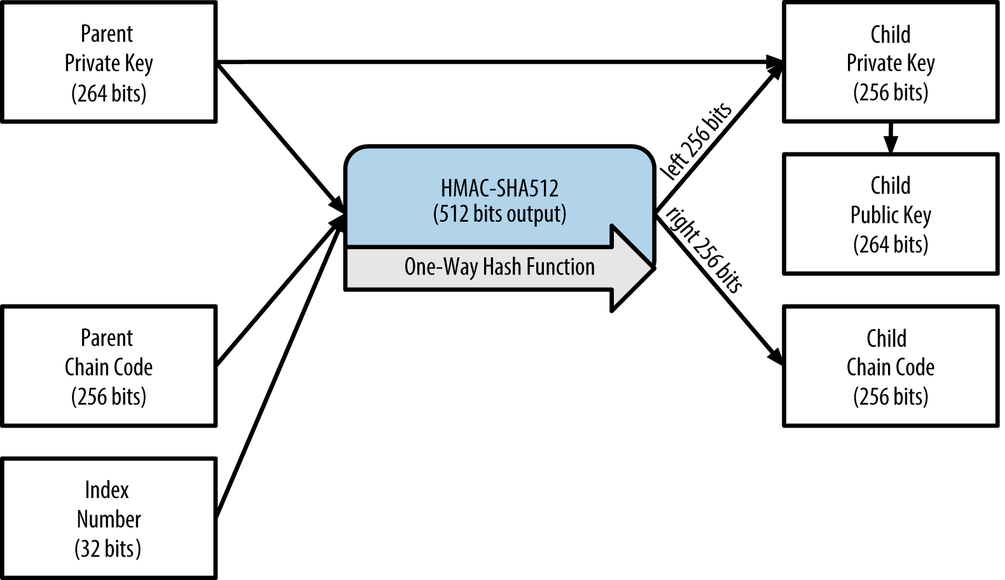
\includegraphics[width=15cm]{Figures/hardened_derivation.png} %cambiare immagine
	\caption{Hardened Derivation }
	\label{fig:pubtopub}
\end{figure}

\subsection{Weakness of Normal Derivation}
As shown above the normal derivation present a great advantage, but also a weakness. It is possible to derive the \textbf{parent extended private key} knowing the \textbf{parent extended public key} and only one of the \textbf{child extended private key}.
\\ \\
The HMAC-SHA256 function has as input three elements: the parent chain code, the parent public key and the child index. The firsts two information can be taken from the parent extended public key, instead the child index can be taken from the child extended private key.

\begin{equation*}
msg = compressed \;parent\; public\;key \;|\;child\; index
\end{equation*}
Then apply the HMAC algorithm with the usual input:

\begin{itemize}[label=$\odot$]
	\item \textbf{Hash function}: SHA512
	\item \textbf{Key}: parent chain code
	\item \textbf{Message}: $msg$
\end{itemize}
Consider the first 32 bytes of the result of this function and consider it as an integer number, $q$.
\\ \\
Remembering that to get the child private key it is needed to compute a sum with the parent private key, it is possible to reverse the process. \\ \\
Let's call $p_{child}$ and $p_{parent}$ the private keys of the child and the father respectively.
\begin{equation}\label{eq3}
\begin{split}
p_{child} &= q+p_{parent} \qquad \mod (order) \\
&\Downarrow \\
p_{parent} &=p_{child}-q \qquad \mod (order)
\end{split}
\end{equation}
The implication \ref{eq3} holds also with modular arithmetic.
\\ \\
So we have derived the private key of the parent. Graphically this derivation can be shown in figure \ref{fig:from_child_to_parent}
\begin{figure}[ht!]
	\centering
	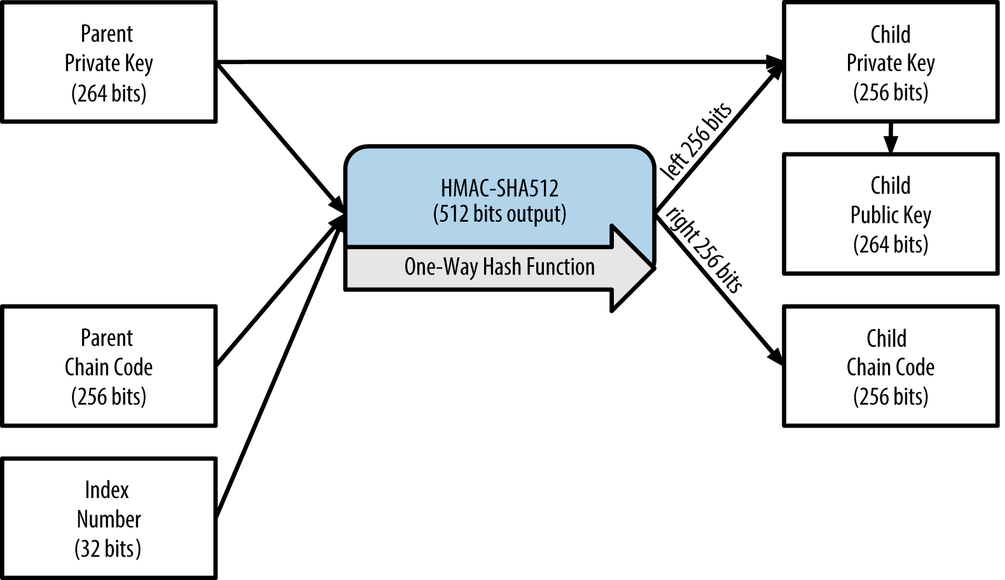
\includegraphics[width=15cm]{Figures/hardened_derivation.png} %cambiare immagine
	\caption{Hardened Derivation }
	\label{fig:from_child_to_parent}
\end{figure}

 

	% Chapter 1

\chapter{Mnemonic phrase} % Main chapter title

\label{mnemonic} % For referencing the chapter elsewhere, use \ref{Chapter1}

%----------------------------------------------------------------------------------------

% Define some commands to keep the formatting separated from the content 
%\newcommand{\keyword}[1]{\textbf{#1}}
%\newcommand{\tabhead}[1]{\textbf{#1}}
%\newcommand{\code}[1]{\texttt{#1}}
%\newcommand{\file}[1]{\texttt{\bfseries#1}}
%\newcommand{\option}[1]{\texttt{\itshape#1}}

%----------------------------------------------------------------------------------------

We have seen how it is possible to generate keys starting from a seed. But a seed is a long number, difficult to remember and not easy to write down on a paper. You may incur typos while transcribing it, and this can compromise the entire wallet.
\begin{remark}
	Mistyping a single digit in the seed produce completely different keys
\end{remark}
In order to work around this problem, some solution were implemented. Among them, the most widespread and used is the one described by BIP39, \textit{Bitcoin Improvement Proposal}. This is not the only one, in this chapter we will also see another solution proposed by Electrum, one of the most famous Bitcoin wallet.
\\ \\
Both these solutions used a \textit{Mnemonic phrase}, from which the seed is obtained. This sentence is designed to avoid typing errors while maintaining the same level of security and entropy.
\begin{flushleft}
	\textbf{What is a Mnemonic phrase?}
\end{flushleft}
A Mnemonic phrase is a set of words taken from a specific dictionary. Although the choice of the dictionary is not binding, the most commonly used among the practitioners is the English one, defined by BIP39. It contains 2048 common words of the English language, each of them from 3 to 9 letters. The set of words that make up the dictionary must be chosen in such a way that the words within it are easy to remember and difficult to misinterpret with one another. It is better to avoid to insert into the dictionary two words with similar meaning or spelling.

\section{BIP39}
First we will see how to generate a mnemonic phrase in the framework of BIP39 and then how it is possible to obtain a seed from it.

\subsection{Mnemonic Generation}
In order to generate a Mnemonic phrase we will start from a given entropy, that can be seen as a large integer number. The way to obtain it can be left free to the user: he can obtain it by inserting arbitrarily chosen numbers (poor choice of randomness), roll a dice many times or with any other method he considers suitable. Many softwares provide a function that generate entropy with quite randomness, but if someone is skeptical about the reliability of software randomness, he must provide himself with such integer number.
\\ \\
Call \textit{ENT} the number of binary digits of the given entropy. Then \textit{ENT} should belongs to a given set:
\begin{equation*}
	ENT \in \{128,160,192,224,256\}
\end{equation*}
The reason for a given length for the entropy will be clear in a moment.
\\ \\
Write the entropy in bytes format, obtaining a string of $ENT/8$ length. Compute the SHA256 algorithm and consider only the first $ENT/32$ bits as a checksum. Finally add these bits to the bottom of the entropy, obtaining an integer number, called \textit{entropy\_checked}, expressed in binary format of length equal to: $ENT+ENT/32$.

\begin{flushleft}
	In python:
\end{flushleft}

\begin{lstlisting}[language=Python]
from hashlib import sha256

entropy_bytes = entropy.to_bytes(int(ENT/8), byteorder='big')
checksum = sha256(entropy_bytes).digest()
entropy_checked = entropy_bin + checksum_bin[:int(ENT/32)]
\end{lstlisting}
Where \textit{entropy\_bin} and \textit{checksum\_bin} are strings of bits that can be concatenated.
\\ \\
Now it is clear the reason for a constraint on the length of the entropy in input: 
\begin{enumerate}[label=\roman*]
	\item \textit{ENT} must be a dividend of 32
	\item $ENT<128$ could be not secure enough.
	\item $ENT>256$ is useless.
\end{enumerate}
The point (i) is due to the structure proposed by BIP39. It is only a convention to take the first $ENT/32$ bits as a checksum. However it is essential that the final length of the entropy plus the checksum must be a dividend of 11, from the moment that the dictionary is a set of $2^{11}$ words.
\\ \\
The point (ii) is just a suggestion because taking less entropy could bring to a leak of security. It will be easier for an attacker to guess your mnemonic phrase by trying out all the possible combinations if less words are involved. It is important to remember that adding even a single bit of entropy, doubles the difficulty of guessing it.
\\ \\
The point (iii) is another suggestion. A private key is a number smaller then $2^{256}$ therefore it would be useless to generate a seed starting from an entropy with more then 256 bits.
\\ \\
Thanks to constraint (i) we obtain that the length of \textit{entropy\_checked} is a dividend of 11:
\begin{equation*}
len(entropy\_checked)=ENT+\dfrac{ENT}{32}=\dfrac{33}{32}\cdot ENT=11\cdot \dfrac{3}{32}\cdot ENT
\end{equation*}
Consider \textit{entropy\_checked} as a string of bits and divide it in substring, each of 11 bits length, obtaining $(\frac{3}{32}\cdot ENT)$ strings of bits.
\\ \\
Each of these strings represents an integer number that can take values in the range between 0 and 2047, ie $2^{11}-1$. Associate each of these numbers with a word in the chosen dictionary, suppose to consider the English one sorted alphabetically. Write down all these words, separated by a space and obtain the Mnemonic Phrase.
\\ \\
An example of Mnemonic Phrase (24 words):
\begin{center}
	\textit{inherit antique flame enrich tell arena eternal floor equal invite swarm pioneer oak benefit giggle damage ship shoe kitten zone shock decline kiss subject}
\end{center}


\subsection{From Mnemonic to Seed}
Once obtaining the Mnemonic phrase we need to derive the seed. In order to do so an hash function is used. So it will be infeasible to derive the Mnemonic phrase from the seed.
\\ \\
The function used is the PBKDF2 and it is used in order to avoid brute force attack, from the moment that the output has exactly the same length of a standard hash function, but it will take more times to calculate it from the moment that it will compute the same hash function many times.
\\ \\

It receives as input:
\begin{itemize}[label=$\odot$]
	\item \textbf{Password}: Mnemonic phrase
	\item \textbf{Salt}: 'mnemonic' + passphrase
	\item \textbf{Number of iterations}: 2048
	\item \textbf{Digest-module}: SHA512
	\item \textbf{Mac-module}: HMAC
\end{itemize}
Summing up it can be said that it calculates the same hash function (HMAC-SHA512) 2048 times.
\\ \\
In order to introduce more complexity in the seed computation a \textit{Salt} is introduced. If not specified the standard salt is simply the world 'mnemonic', otherwise it could be extended with an optional \textit{passphrase}.
\\ \\
Although it is true that a human being is a scarce source of randomness, the passphrase is usually chosen by the user. This is due to the fact that it has a different purpose to the mnemonic phrase. We will analyze some useful applications in the next chapter. 
\begin{remark}
	The randomness should be guaranteed by the input entropy used to generate the mnemonic phrase, not by the passphrase.
\end{remark}
The python code is the follow:
\begin{lstlisting}[language=Python]
from hashlib import sha512
from pbkdf2 import PBKDF2
import hmac

seed = PBKDF2(mnemonic, 'mnemonic' + passphrase, iterations = 2048, macmodule = hmac, digestmodule = sha512).read(64)
\end{lstlisting}
Where \textit{mnemonic} is the mnemonic phrase previously computed and \textit{passphrase} is chosen by the user

\begin{remark}
	With this procedure we always produce a seed of specific length: 512 bits. It will always be enough because every private key can take value from a smaller set of value (1 to \textit{order}).
\end{remark}

\section{Electrum Mnemonic}
Even if BIP39 is proposed, it is not the only solution adopted among the practitioners. One example is the one proposed by Electrum.
\\ \\
The main difference is in the way that the mnemonic phrase is generated and the purpose of it. Electrum choses to assign a version to the seed in such a way that is possible to recognize the purpose of the key generated from it.

\subsection{Mnemonic and Seed Generation}
Whenever a new mnemonic phrase is required, Electrum starts from an given entropy, generated through a random function. Obviously it is possible to generate a valid mnemonic phrase with an entropy chosen by the user, if he is skeptical or doesn't want to relay on the reliability of the randomness of a random function.
\\ \\
To be consistent, call \textit{ENT} the number of binary digits of the given entropy. Then \textit{ENT} must be a multiple of 11. 






	% Chapter 1

\chapter{How to use a HD Wallet} % Main chapter title

\label{bip32} % For referencing the chapter elsewhere, use \ref{Chapter1}

%----------------------------------------------------------------------------------------

% Define some commands to keep the formatting separated from the content 
%\newcommand{\keyword}[1]{\textbf{#1}}
%\newcommand{\tabhead}[1]{\textbf{#1}}
%\newcommand{\code}[1]{\texttt{#1}}
%\newcommand{\file}[1]{\texttt{\bfseries#1}}
%\newcommand{\option}[1]{\texttt{\itshape#1}}

%----------------------------------------------------------------------------------------

\section{BIP 44}





	% Chapter 1

\chapter*{Conclusion} % Main chapter title
\addcontentsline{toc}{chapter}{Conclusion}
\label{Conclusion} % For referencing the chapter elsewhere, use \ref{Chapter1} 

%----------------------------------------------------------------------------------------

% Define some commands to keep the formatting separated from the content 
%----------------------------------------------------------------------------------------
The main purpose of this thesis was the analysis of the principal methods used to generate private and public keys and to store the seed. 
\\ \\
First we briefly described some simple deterministic derivation, then we analyzed the Hierarchical Deterministic Wallet. It was possible to derive an extended key in two way: normal and hardened. The use of the normal derivation allowed the user to derive also the public key from an extended public key, but the entire wallet could be compromised if the parent extended public key and a child extended private key were stolen. The use of the hardened derivation prevented this problem, with the cons to not allow the public to public derivation. 
\\ \\
Then we focused on the two methods mostly used to generate the seed: the version proposed by BIP39 and the one proposed by Electrum. Both of them started from a given entropy, from which a mnemonic phrase was generated and from the latter, the seed was obtained. This two method were very similar, but they had some subtle differences. In this thesis, these differences were deeply analyzed, showing all the pros and cons of each method. 
\\ \\
It is not the purpose of this work to point out a better proposal, but to give a complete and detailed overview of the various way to generate your keys. 
\vfill
\textit{"We often fear what we do not understand. Our best defense is knowledge."}
\begin{flushright}
	Lieutenant Tuvok, Star Trek: Voyager
\end{flushright}


	
	%----------------------------------------------------------------------------------------
	%	THESIS CONTENT - APPENDICES
	%----------------------------------------------------------------------------------------
	
	\appendix % Cue to tell LaTeX that the following "chapters" are Appendices
	
	% Include the appendices of the thesis as separate files from the Appendices folder
	% Uncomment the lines as you write the Appendices
	
	% Appendix A

\chapter{Frequently Asked Questions} % Main appendix title

\label{AppendixA} % For referencing this appendix elsewhere, use \ref{AppendixA}

\section{How do I change the colors of links?}

The color of links can be changed to your liking using:

{\small\verb!\hypersetup{urlcolor=red}!}, or

{\small\verb!\hypersetup{citecolor=green}!}, or

{\small\verb!\hypersetup{allcolor=blue}!}.

\noindent If you want to completely hide the links, you can use:

{\small\verb!\hypersetup{allcolors=.}!}, or even better: 

{\small\verb!\hypersetup{hidelinks}!}.

\noindent If you want to have obvious links in the PDF but not the printed text, use:

{\small\verb!\hypersetup{colorlinks=false}!}.

	%\include{Appendices/AppendixB}
	%\include{Appendices/AppendixC}
	
	%----------------------------------------------------------------------------------------
	%	BIBLIOGRAPHY
	%----------------------------------------------------------------------------------------
	
	\begin{thebibliography}{12}
		\bibitem{1}
		\href{https://github.com/bitcoin/bips/blob/master/bip-0032.mediawiki}{BIP32, Bitcoin Improvement Proposal number 32 \\ \texttt{https://github.com/bitcoin/bips/blob/master/bip-0032.mediawiki}}
		
		\bibitem{2}
		\href{https://github.com/bitcoin/bips/blob/master/bip-0039.mediawiki}{BIP39, Bitcoin Improvement Proposal number 39 \\ \texttt{https://github.com/bitcoin/bips/blob/master/bip-0039.mediawiki}}
		
		
		\bibitem{3} 
		\href{https://electrum.org}{Electrum Bitcoin Wallet \\ \texttt{https://electrum.org}}
		
		\bibitem{4} 
		\href{https://github.com/bitcoin/bips/blob/master/bip-0043.mediawiki}{BIP43, Bitcoin Improvement Proposal number 43 \\ \texttt{https://github.com/bitcoin/bips/blob/master/bip-0043.mediawiki}}

		\bibitem{5}
		\href{https://github.com/bitcoin/bips/blob/master/bip-0044.mediawiki}{BIP44, Bitcoin Improvement Proposal number 44 \\ \texttt{https://github.com/bitcoin/bips/blob/master/bip-0044.mediawiki}}
		
		\bibitem{6} 
		\href{https://github.com/bitcoin/bips/blob/master/bip-0049.mediawiki}{BIP49, Bitcoin Improvement Proposal number 49 \\ \texttt{https://github.com/bitcoin/bips/blob/master/bip-0049.mediawiki}}
		
		\bibitem{7} 
		\href{https://github.com/bitcoinbook/bitcoinbook}{Andreas M. Antonopoulos, \textit{Mastering Bitcoin 2nd Edition - Programming the Open Blockchain}. 2017.}
		
		\bibitem{8} 
		\href{http://andrea.corbellini.name}{Andrea Corbellini, \texttt{http://andrea.corbellini.name}}
		
		\bibitem{9} 
		Bundesamt fur Sicherheit in der Informationstechnik, \textit{Elliptic Curve Cryptography}, 2007.
		
		\bibitem{10} 
		Christof Paar, Jan Pelzl, \textit{Understanding Cryptography}, 2010.
		
		\bibitem{11} 
		\href{https://bitcoin.org/bitcoin.pdf}{Satoshi Nakamoto, \textit{Bitcoin: A Peer-to-Peer Electronic Cash System}, 2008.}
		
		\bibitem{12} 
		\href{https://bitcoincore.org}{Bitcoin Core, \texttt{https://bitcoincore.org}}
		

	\end{thebibliography}

%\bibliographystyle{unsrt}
%\bibliography{bibliography}
	
	\printbibliography[heading=bibintoc]
	
	%----------------------------------------------------------------------------------------
	
\end{document}  
